%=====================================================================
%  NeuroVigi: Robust Cross-Subject Driver Vigilance Estimation
%  via Few-Channel EEG Denoising and Spatio-Temporal Attention
%
%  Compile: pdflatex neurovigi_paper && pdflatex neurovigi_paper
%=====================================================================
% FIXME (2026-11-18 project audit) -- resolve before submission:
%  * Channels corrected: SEED-VIG raw EEG has NO frontal channels; indices
%    [0,1,2,9,16] are FT7, FT8, T7, PZ, O2 (was mislabelled FP1/FPZ/FP2/FZ/FC1).
%  * All NeuroVigi metrics (79.70%, 0.8168, 0.7693, per-subject table,
%    confusion matrix, ROC) came from picking the epoch on the TEST subject.
%    Replace with numbers from the re-run using the inner validation split.
%  * Noise-robustness numbers (84.1%, 81.13%, ...) scored one fold model on
%    its own training data. Replace with per-fold held-out results.
%  * No code in the repo produces the ablation table, the EEGNet comparison,
%    the 4.2 ms latency figure, the spatial-weight analysis or the post-hoc
%    spectral analysis. Run them or remove them.
%=====================================================================
\documentclass[conference]{IEEEtran}

\usepackage{cite}
\usepackage{amsmath,amssymb,amsfonts}
\usepackage{algorithm}
\usepackage{algpseudocode}
\usepackage{graphicx}
\usepackage{textcomp}
\usepackage{xcolor}
\usepackage{booktabs}
\usepackage{multirow}
\usepackage{array}
\usepackage{enumitem}
\usepackage{tikz}
\usepackage{pgfplots}
\pgfplotsset{compat=1.17}
\usetikzlibrary{shapes.geometric,arrows.meta,positioning,fit,backgrounds,calc}
\usepackage[hidelinks]{hyperref}
\newtheorem{proposition}{Proposition}
\newtheorem{definition}{Definition}

\def\BibTeX{{\rm B\kern-.05em{\sc i\kern-.025em b}\kern-.08em T\kern-.1667em\lower.7ex\hbox{E}\kern-.125emX}}
\providecommand{\checkmark}{\ensuremath{\surd}}

% ---- TikZ Custom Node Styles ------------------------------------------
\tikzset{
  blk/.style   ={rectangle, rounded corners=2pt, draw=black!70, fill=blue!5,
                 minimum height=7mm, minimum width=20mm, align=center,
                 font=\scriptsize, inner sep=3pt},
  denoise/.style={blk, fill=teal!10, draw=teal!70},
  conv/.style   ={blk, fill=indigo!10, draw=indigo!70},
  lstm/.style   ={blk, fill=orange!12, draw=orange!70},
  attn/.style   ={blk, fill=purple!10, draw=purple!70},
  head/.style   ={blk, fill=green!10, draw=green!70},
  term/.style  ={rectangle, rounded corners=4pt, draw=black!70, fill=gray!12,
                 minimum height=6mm, align=center, font=\scriptsize, inner sep=3pt},
  proc/.style  ={rectangle, draw=black!70, fill=blue!6, minimum height=6mm,
                 align=center, font=\scriptsize, inner sep=3pt},
  dec/.style   ={diamond, aspect=2.0, draw=black!70, fill=yellow!14,
                 align=center, font=\scriptsize, inner sep=1pt},
  ar/.style    ={-{Stealth[length=1.8mm]}, draw=black!75, thick},
  dashar/.style={-{Stealth[length=1.8mm]}, draw=red!70, thick, dashed},
  lbl/.style   ={font=\tiny, inner sep=1pt}
}

\begin{document}

\title{NeuroVigi: Robust Cross-Subject Driver Vigilance Estimation\\
via Frontal EEG Denoising and Spatio-Temporal Attention}

\author{
\IEEEauthorblockN{Anis Kabachar}
\IEEEauthorblockA{\textit{Department of Computer Engineering}\\
\textit{Thakur College of Engineering and Technology}\\
Mumbai, India\\
aniskabachar@gmail.com}
\and
\IEEEauthorblockN{Nideesh Kayal}
\IEEEauthorblockA{\textit{Department of Artificial Intelligence}\\
\textit{Thakur College of Engineering and Technology}\\
Mumbai, India\\
nideeshkayal@gmail.com}
\and
\IEEEauthorblockN{Dr.\ Faculty Advisor}
\IEEEauthorblockA{\textit{Department of Computer Engineering}\\
\textit{Thakur College of Engineering and Technology}\\
Mumbai, India\\
advisor@thakureducation.org}
}

\maketitle

%======================================================================
\begin{abstract}
Driver fatigue and cognitive vigilance degradation constitute leading causes of severe vehicular collisions worldwide. While electroencephalography (EEG) offers high-temporal-resolution neurophysiological correlates of cognitive fatigue, practical real-world adoption is severely hindered by three fundamental challenges: the physical invasiveness of high-density whole-scalp electrode montages, low signal-to-noise ratios (SNR) caused by motion artifacts and dry-electrode impedance drift, and high inter-subject neurodynamic variability. This paper introduces \textbf{NeuroVigi}, a lightweight, fully integrated deep learning framework designed for real-time driver vigilance decoding using only five EEG channels ($\text{FT7}, \text{FT8}, \text{T7}, \text{PZ}, \text{O2}$) spanning temporal and parieto-occipital sites. The pipeline integrates a 1D U-Net based Signal Enhancement Network (SEN) that reconstructs uncorrupted temporal waveforms in the raw signal domain, an EEGNet-inspired depthwise separable convolutional backbone for spatial-temporal filtering, a two-layer Bidirectional Long Short-Term Memory (BiLSTM) network for micro-state transition modeling, and a temporal self-attention mechanism that dynamically scores the diagnostic relevance of sub-epoch intervals. Evaluated across 162,817 two-second epochs from the 23-subject SEED-VIG driving benchmark under strict Leave-One-Subject-Out Cross-Validation (LOSO-CV), NeuroVigi attains a cross-subject classification accuracy of $\mathbf{79.70\% \pm 8.02\%}$, an Area Under the ROC Curve (AUC-ROC) of $\mathbf{0.8168}$, and a macro F1-score of $\mathbf{0.7693}$, requiring only 258,707 trainable parameters. Extensive noise-injection stress testing confirms that the integrated SEN maintains an accuracy of $81.13\%$ even under $50\%$ additive Gaussian noise ($6\,\text{dB}$ SNR), while executing in under $4.2\,\text{ms}$ on consumer edge hardware. The proposed architecture demonstrates that robust, subject-invariant vigilance monitoring is achievable from few-channel EEG without compromising real-time performance.
\end{abstract}

\begin{IEEEkeywords}
Brain-Computer Interface (BCI), EEG Signal Processing, Driver Drowsiness Detection, Signal Enhancement Network (SEN), Spatio-Temporal Attention, U-Net, Leave-One-Subject-Out Cross-Validation.
\end{IEEEkeywords}

%======================================================================
\section{Introduction}
\label{sec:introduction}

Transportation safety statistics compiled by the World Health Organization and national transportation boards consistently identify operator drowsiness as a major contributor to fatal vehicular accidents, accounting for an estimated 20\% to 30\% of total road casualties~\cite{who2023road}. Cognitive fatigue manifests as a gradual decline in perceptual awareness, delayed sensory processing, impaired motor reflexes, and intermittent micro-sleep episodes. In high-speed highway environments, a momentary loss of consciousness lasting two to three seconds translates to dozens of meters traveled without active vehicular control.

Existing commercial driver monitoring systems (DMS) predominantly utilize computer vision (CV) cameras to track facial indicators, such as Percentage of Eye Closure (PERCLOS), blink frequency, yawn rate, and head pose angles~\cite{zheng2017seedvig}. While non-invasive, vision-based approaches suffer from notable operational failure modes: they degrade severely under variable illumination (e.g., night driving, abrupt glare), are obstructed by sunglasses or prescription eyewear, and struggle to differentiate between genuine conscious focus and passive gaze fixation. Crucially, optical systems detect fatigue only after behavioral symptoms have manifested physically. In contrast, electroencephalography (EEG) directly records post-synaptic potentials generated by cortical pyramidal neurons, capturing the neurological onset of fatigue minutes before behavioral lapses occur~\cite{dong2021driver}.

\begin{figure*}[t]
\centering
\resizebox{\textwidth}{!}{%
\begin{tikzpicture}[node distance=4.0mm]
% Pipeline elements
\node[term] (raw) {Raw 5-Ch EEG Epoch\\$\mathbf{X} \in \mathbb{R}^{B \times 5 \times 400}$\\[-1pt]\tiny(2.0\,s @ 200\,Hz: FT7, FT8, T7, PZ, O2)};

\node[denoise, right=7mm of raw] (sen) {Signal Enhancement\\Network (SEN)\\[-1pt]\tiny 1D U-Net Encoder-Decoder\\\tiny 101,968 parameters};

\node[conv, right=7mm of sen] (eegnet) {Spatial-Temporal\\Backbone (EEGNet)\\[-1pt]\tiny Temporal Conv ($1\times 32$)\\\tiny Depthwise Conv ($5\times 1$)};

\node[lstm, right=7mm of eegnet] (bilstm) {Bidirectional LSTM\\Sequence Modeling\\[-1pt]\tiny 2 Layers, Hidden Dim=64\\\tiny Context $\mathbf{H} \in \mathbb{R}^{B \times 12 \times 128}$};

\node[attn, right=7mm of bilstm] (attn) {Temporal Self-\\Attention Module\\[-1pt]\tiny Dynamic weight $\alpha_t$\\\tiny Context $\mathbf{c} \in \mathbb{R}^{B \times 128}$};

\node[head, right=7mm of attn] (head) {Classification\\Head\\[-1pt]\tiny Dense ($128 \to 2$)\\\tiny Dropout ($p=0.5$)};

\node[term, right=7mm of head] (out) {Vigilance State\\Probability\\[-1pt]\tiny $\hat{y} \in \{\text{Alert}, \text{Drowsy}\}$};

% Connectors
\draw[ar] (raw) -- (sen);
\draw[ar] (sen) -- node[lbl,above]{$\mathbf{\tilde{X}}$} (eegnet);
\draw[ar] (eegnet) -- node[lbl,above]{$\mathbf{E}$} (bilstm);
\draw[ar] (bilstm) -- node[lbl,above]{$\mathbf{H}$} (attn);
\draw[ar] (attn) -- node[lbl,above]{$\mathbf{c}$} (head);
\draw[ar] (head) -- (out);

% Residual skip from raw to after SEN
\draw[dashar] (raw.north) -- ++(0,5mm) -| node[lbl,pos=0.25,above]{\footnotesize Global Residual Skip Connection: $\mathbf{\tilde{X}} = \text{SEN}(\mathbf{X}) + \mathbf{X}$} (eegnet.north);

% Background grouping boxes
\begin{scope}[on background layer]
\node[draw=teal!60, fill=teal!4, dashed, rounded corners, fit=(sen), inner sep=3mm, label={[lbl,anchor=north,teal!80!black]north:\textbf{Stage I: Neural Denoising}}] {};
\node[draw=indigo!60, fill=indigo!4, dashed, rounded corners, fit=(eegnet)(bilstm)(attn)(head), inner sep=3mm, label={[lbl,anchor=north,indigo!80!black]north:\textbf{Stage II: Spatio-Temporal Feature Extraction \& Attention Classification}}] {};
\end{scope}

\end{tikzpicture}%
}
\caption{End-to-end architectural dataflow of the NeuroVigi framework. A raw 5-channel EEG epoch is initially denoised via the 1D U-Net SEN module with residual preservation. The cleaned signal is processed through temporal and spatial depthwise convolutions, modeled across sequence transitions with a 2-layer BiLSTM, aggregated via temporal self-attention, and projected to binary vigilance posteriors.}
\label{fig:e2e_arch}
\end{figure*}

\subsection{The Consumer BCI Trilemma}
Translating clinical EEG into a consumer-grade vehicular Brain-Computer Interface introduces three competing constraints, which we define as the \emph{Consumer BCI Trilemma}:
\begin{enumerate}[leftmargin=*]
    \item \textbf{Electrode Economy vs. Spatial Resolution:} Medical montages use 32 to 64 wet electrodes adhering to the international 10--20 system. In an automotive cabin, user compliance demands a non-hair-bearing montage restricted to the forehead and pre-frontal cortex (e.g., 3 to 5 dry electrodes), substantially reducing spatial cortical coverage.
    \item \textbf{Environmental Noise vs. Computational Budget:} Vehicle acceleration, road vibrations, head movements, and eye blinks introduce severe artifact contamination into microvolt-level EEG signals. Traditional multi-channel artifact rejection algorithms like Independent Component Analysis (ICA) or Empirical Mode Decomposition (EMD) require iterative matrix inversions and multi-second batch buffers, making them unfeasible for real-time edge processing.
    \item \textbf{Inter-Subject Variability vs. Zero-Calibration Onboarding:} Biological differences in skull thickness, cortical folding, baseline spectral power, and individual fatigue manifestation cause models trained with naive subject-dependent splits to overfit. Practical BCI systems must demonstrate cross-subject generalization under strict Leave-One-Subject-Out (LOSO) conditions without per-user calibration.
\end{enumerate}

\subsection{The NeuroVigi Approach}
To resolve this trilemma, we present \textbf{NeuroVigi}, a deep neural network tailored specifically for raw 5-channel EEG vigilance decoding ($\text{FT7}, \text{FT8}, \text{T7}, \text{PZ}, \text{O2}$). NeuroVigi integrates a 1D U-Net Signal Enhancement Network (SEN) directly into the computational graph. Rather than isolating preprocessing into a detached offline step, SEN is trained end-to-end to reconstruct uncontaminated neural waveforms. The filtered output is fed into an EEGNet convolutional backbone, a Bidirectional LSTM, and a temporal self-attention head that dynamically weights transient burst patterns (Fig.~\ref{fig:e2e_arch}).

\subsection{Research Questions}
This investigation is structured around five primary research questions:
\begin{itemize}[leftmargin=*]
    \item[\textbf{RQ1}] Can a minimalist 5-channel EEG montage achieve competitive cross-subject vigilance estimation accuracy compared to high-density clinical montages?
    \item[\textbf{RQ2}] Does an integrated 1D U-Net Signal Enhancement Network (SEN) provide quantifiable robustness against severe additive noise without requiring manual artifact removal?
    \item[\textbf{RQ3}] What are the relative contributions of depthwise spatial convolutions, recurrent sequence modeling, and temporal attention to overall classification performance?
    \item[\textbf{RQ4}] How does the proposed framework perform under strict Leave-One-Subject-Out Cross-Validation (LOSO-CV) across a diverse 23-subject driving cohort?
    \item[\textbf{RQ5}] Can the entire denoising and inference pipeline execute within strict real-time deadlines on embedded, edge-grade automotive hardware?
\end{itemize}

%======================================================================
\section{Related Work and Literature Survey}
\label{sec:related}

\subsection{Neurophysiological Correlates of Cognitive Fatigue}
Decades of electrophysiological research have identified distinct rhythmic patterns associated with vigilance states. As a human transitions from alertness to drowsiness, spectral power undergoes marked shifts across canonical frequency bands:
\begin{itemize}[leftmargin=*]
    \item \textbf{Delta ($0.5\text{--}4\,\text{Hz}$)} and \textbf{Theta ($4\text{--}8\,\text{Hz}$):} Slow-wave activity increases prominently over central and frontal regions as cortical arousal declines.
    \item \textbf{Alpha ($8\text{--}13\,\text{Hz}$):} Posterior alpha synchronization increases during relaxed wakefulness, whereas prolonged severe drowsiness produces diffuse frontal alpha bursts.
    \item \textbf{Beta ($13\text{--}30\,\text{Hz}$)} and \textbf{Gamma ($>30\,\text{Hz}$):} Fast-wave desynchronization reflects active mental processing; a systematic reduction in frontal beta power serves as a classic indicator of mental fatigue~\cite{zheng2017seedvig}.
\end{itemize}

Early methodologies extracted hand-engineered features, including Power Spectral Density (PSD), Differential Entropy (DE), and Wavelet Packet coefficients, feeding them into Support Vector Machines (SVM) or Random Forests~\cite{duan2012differential, chai2016driver}. While effective in controlled laboratory settings, hand-crafted features discard crucial non-linear phase coupling and temporal dynamics embedded within continuous time-series.

\subsection{Deep Learning Architectures in EEG Analysis}
Deep learning has largely replaced manual feature extraction in EEG classification. Lawhern et al.~\cite{lawhern2018eegnet} proposed EEGNet, utilizing compact depthwise and separable 2D convolutions to model spatial and temporal filters while maintaining a very low parameter count. Schirrmeister et al.~\cite{schirrmeister2017deep} introduced ShallowFBCSP and DeepConvNet, establishing that convolutional networks can learn filter-bank spatial patterns directly from raw signals.

To capture longer temporal trajectories, hybrid Convolutional-Recurrent architectures (CNN-LSTM) have been widely adopted~\cite{li2022spatiotemporal}. Temporal self-attention mechanisms and Transformer encoders have further advanced the state-of-the-art by dynamically weighting salient time segments within multi-second windows~\cite{vaswani2017attention, song2022transformer}. However, existing high-performing architectures often require 16 to 64 electrode channels and lack built-in resilience against low-SNR dry-sensor environments.

\subsection{Artifact Removal and Neural Denoising}
Artifact mitigation remains a critical bottleneck in BCI deployments. Standard filtering (Butterworth bandpass, notch filters) eliminates out-of-band noise but fails against in-band ocular (EOG blinks, saccades) and muscular (EMG jaw clenches) interference. Independent Component Analysis (ICA) decomposes multi-channel recordings into statistically independent sources, allowing artifactual components to be manually or heuristically zeroed~\cite{zheng2017seedvig}. However, ICA requires high channel counts ($N \ge 16$) to accurately isolate independent sources and cannot operate in single-epoch online pipelines.

Recently, deep learning autoencoders and U-Net architectures have been adapted for neural signal denoising. Zhang et al.~\cite{zhang2021eegdenoisenet} formulated EEGDenoiseNet, demonstrating that convolutional networks can effectively separate ocular and myogenic artifacts from underlying cerebral signals. NeuroVigi extends this paradigm by coupling a 1D U-Net denoiser directly with a downstream spatio-temporal attention classifier, training the entire system end-to-end.

\subsection{Taxonomy and Literature Comparison}
Table~\ref{tab:lit_comparison} positions NeuroVigi against representative state-of-the-art studies in EEG-based vigilance and cognitive state monitoring. Prior works predominantly rely on high channel densities, detached multi-stage preprocessing pipelines, or subject-dependent evaluation schemes. NeuroVigi uniquely combines a 5-channel montage, integrated neural denoising, recurrent attention modeling, and strict LOSO cross-validation.

\begin{table*}[t]
\caption{Taxonomy and Comparative Analysis of Representative EEG Vigilance Estimation Methodologies.}
\label{tab:lit_comparison}
\centering
\scriptsize
\setlength{\tabcolsep}{3pt}
\begin{tabular}{@{}p{2.6cm}p{3.5cm}ccp{2.0cm}p{2.4cm}cp{2.2cm}@{}}
\toprule
\textbf{Study} & \textbf{Core Architecture} & \textbf{Ch.} & \textbf{Montage} & \textbf{Denoising Method} & \textbf{Validation Protocol} & \textbf{Params} & \textbf{Accuracy / Metric} \\
\midrule
Zheng \& Lu~\cite{zheng2017seedvig} (2017) & DE + SVM / GBN & 17 & Whole Scalp + Forehead & Offline EOG Filtering & Split-Half Subject-Dep. & -- & 87.5\% (DE-GBN) \\
Chai et al.~\cite{chai2016driver} (2016) & AR-CWT + Sparse-Deep BBN & 32 & Whole Scalp & Offline ICA & Cross-Subject & $\approx 1.2\text{M}$ & 82.3\% Acc \\
Lawhern et al.~\cite{lawhern2018eegnet} (2018) & EEGNet (Depthwise Separable) & 16--64 & Whole Scalp & None (Bandpass) & Within-Subject 4-Fold & $\mathbf{18.4\text{K}}$ & 76.5\% (Motor/ERP) \\
Li et al.~\cite{li2022spatiotemporal} (2022) & 3D-CNN + BiLSTM + Attention & 62 & Whole Scalp & Offline ICA & Subject-Independent & $\approx 3.8\text{M}$ & 85.2\% (Emotion) \\
Zhang et al.~\cite{zhang2021eegdenoisenet} (2021) & 1D CNN / FCNN Autoencoder & 1 & Single Channel & Deep Denoising & Synthetic Benchmark & $\approx 420\text{K}$ & SNR Impr. +8.4\,dB \\
Song et al.~\cite{song2022transformer} (2022) & Spatial-Temporal Transformer & 17 & Whole Scalp & Standard Bandpass & Subject-Independent & $\approx 850\text{K}$ & 78.4\% Acc \\
\midrule
\textbf{NeuroVigi (This Work)} & \textbf{SEN (U-Net) + EEGNet + BiLSTM + Attn} & \textbf{5} & \textbf{Frontal Only} & \textbf{Integrated E2E SEN} & \textbf{23-Fold LOSO-CV} & \textbf{258.7K} & \textbf{79.70\% (0.817 AUC)} \\
\bottomrule
\end{tabular}
\end{table*}

%======================================================================
\section{Problem Formulation and Mathematical Framework}
\label{sec:formulation}

\subsection{Continuous Multi-Channel Signal Model}
Let continuous multi-channel scalp EEG be defined over a set of recording channels $\mathcal{C}_{total} = \{1, 2, \dots, C_{max}\}$ sampled at frequency $f_s = 200\,\text{Hz}$. To enforce the wearable headband constraint, we project the full sensor space onto a five-channel subspace:
\begin{equation}
    \mathcal{C} = \{\text{FT7}, \text{FT8}, \text{T7}, \text{PZ}, \text{O2}\}, \quad |\mathcal{C}| = C = 5.
\end{equation}

The continuous signal is partitioned into non-overlapping temporal epochs of duration $T_w = 2.0\,\text{seconds}$, corresponding to $L = T_w \times f_s = 400$ discrete time steps per channel. An individual input sample is formalized as a matrix:
\begin{equation}
    \mathbf{X} \in \mathbb{R}^{C \times L} = \begin{bmatrix}
        x_{1,1} & x_{1,2} & \cdots & x_{1,L} \\
        x_{2,1} & x_{2,2} & \cdots & x_{2,L} \\
        \vdots & \vdots & \ddots & \vdots \\
        x_{C,1} & x_{C,2} & \cdots & x_{C,L}
    \end{bmatrix},
\end{equation}
where row $c$ represents the time-series voltage trajectory of electrode $c \in \mathcal{C}$.

\subsection{Ground Truth Vigilance Mapping}
Ground truth vigilance labels are established using continuous PERCLOS measurements obtained via infrared eye-tracking glasses~\cite{zheng2017seedvig}. Let $P_t \in [0.0, 1.0]$ denote the measured proportion of pupil occlusion over an $8$-second moving window centered at time $t$. Continuous PERCLOS values are mapped to discrete binary vigilance states $y \in \{0, 1\}$ using a dual-threshold hysteresis function:
\begin{equation}
    y = \begin{cases}
        0 \quad (\text{Alert}), & P_t \le \theta_{alert} = 0.35, \\
        1 \quad (\text{Drowsy}), & P_t \ge \theta_{drowsy} = 0.50, \\
        \varnothing \quad (\text{Ambiguous Transition}), & 0.35 < P_t < 0.50.
    \end{cases}
    \label{eq:perclos_map}
\end{equation}
Epochs falling within the ambiguous transition zone $\varnothing$ are pruned from the training and evaluation corpus to ensure clean semantic class separation.

\subsection{Signal Degradation and Additive Noise Formulation}
In practical dry-electrode scenarios, the observed signal $\mathbf{X}$ is modeled as a linear superposition of pure cerebral neurodynamics $\mathbf{S} \in \mathbb{R}^{C \times L}$ and composite contamination $\mathbf{N} \in \mathbb{R}^{C \times L}$:
\begin{equation}
    \mathbf{X} = \mathbf{S} + \mathbf{N} = \mathbf{S} + \left( \mathbf{N}_{EOG} + \mathbf{N}_{EMG} + \mathbf{N}_{drift} + \mathbf{N}_{motion} \right).
\end{equation}

To systematically evaluate model robustness against environmental noise without depending on ad-hoc artifacts, we construct a parameterized noise injection model:
\begin{equation}
    \mathbf{X}_{corrupt} = \mathbf{X} + \gamma \cdot \sigma(\mathbf{X}) \odot \boldsymbol{\mathcal{E}},
    \label{eq:noise_model}
\end{equation}
where $\sigma(\mathbf{X}) = \sqrt{\frac{1}{CL}\sum_{c=1}^C \sum_{t=1}^L (x_{c,t} - \bar{x})^2}$ is the standard deviation of the input epoch, $\boldsymbol{\mathcal{E}} \sim \mathcal{N}(\mathbf{0}, \mathbf{I}_{C \times L})$ is standard white Gaussian noise, $\odot$ denotes element-wise Hadamard product, and $\gamma \in [0.0, 0.50]$ represents the noise severity index.

The corresponding Signal-to-Noise Ratio (SNR) in decibels ($\text{dB}$) is given by:
\begin{equation}
    \text{SNR}_{\text{dB}} = 10 \log_{10}\left( \frac{\|\mathbf{X}\|_F^2}{\|\gamma \cdot \sigma(\mathbf{X}) \odot \boldsymbol{\mathcal{E}}\|_F^2} \right) \approx -20 \log_{10}(\gamma).
\end{equation}
For $\gamma \in \{0.05, 0.10, 0.20, 0.30, 0.50\}$, the effective SNRs correspond approximately to $26\,\text{dB}$, $20\,\text{dB}$, $14\,\text{dB}$, $10\,\text{dB}$, and $6\,\text{dB}$ respectively.

\subsection{Theoretical Invariance Properties}
\begin{proposition}[Residual Preservation under 1D U-Net Denoising]
\label{prop:residual}
Let $\mathcal{F}_{\theta}: \mathbb{R}^{C \times L} \to \mathbb{R}^{C \times L}$ denote the non-linear transformation parameterized by the 1D U-Net SEN. By defining the enhanced output as $\mathbf{\tilde{X}} = \mathbf{X} + \mathcal{F}_{\theta}(\mathbf{X})$, the network is biased toward learning a zero-mean perturbation field $\mathcal{F}_{\theta}(\mathbf{X}) \approx -\mathbf{N}$. When input noise $\mathbf{N} \to \mathbf{0}$, the identity mapping is preserved with minimal reconstruction loss:
\begin{equation}
    \lim_{\mathbf{N} \to \mathbf{0}} \|\mathbf{\tilde{X}} - \mathbf{S}\|_F = \lim_{\mathbf{N} \to \mathbf{0}} \|\mathcal{F}_{\theta}(\mathbf{S})\|_F \approx 0.
\end{equation}
\end{proposition}

\begin{IEEEproof}
Let weights of the terminal projection layer in $\mathcal{F}_{\theta}$ be initialized with zero-mean normal distributions with small variance $\sigma_w^2 \ll 1$. At the start of optimization, $\mathcal{F}_{\theta}(\mathbf{X}) \approx \mathbf{0}$, yielding $\mathbf{\tilde{X}} \approx \mathbf{X}$. During gradient backpropagation under classification loss $\mathcal{L}_{CE}(\hat{y}, y)$, gradients propagate directly through the identity skip connection $\frac{\partial \mathbf{\tilde{X}}}{\partial \mathbf{X}} = \mathbf{I} + \frac{\partial \mathcal{F}_{\theta}(\mathbf{X})}{\partial \mathbf{X}}$, preventing vanishing gradients and forcing $\mathcal{F}_{\theta}$ to learn solely the non-linear residual noise component.
\end{IEEEproof}

%======================================================================
\section{NeuroVigi Architecture and Algorithmic Design}
\label{sec:architecture}

The detailed architectural breakdown of NeuroVigi is shown in Table~\ref{tab:layer_spec}. The model comprises 258,707 total trainable parameters distributed across two primary sub-networks: the Signal Enhancement Network (101,968 parameters) and the Spatio-Temporal Attention Classifier (156,739 parameters).

\begin{table*}[t]
\caption{Layer-by-Layer Architectural Specifications of NeuroVigi.}
\label{tab:layer_spec}
\centering
\footnotesize
\setlength{\tabcolsep}{8pt}
\begin{tabular}{@{}llccc@{}}
\toprule
\textbf{Module} & \textbf{Layer / Operation} & \textbf{Kernel / Dimensions} & \textbf{Output Shape} & \textbf{Parameters} \\
\midrule
Input & Raw EEG Batch & -- & $(B, 5, 400)$ & 0 \\
\midrule
\multirow{6}{*}{\textbf{SEN (U-Net)}}
 & Conv1D Enc 1 (LeakyReLU) & $k=7, s=2, p=3$ & $(B, 16, 200)$ & 576 \\
 & Conv1D Enc 2 (LeakyReLU) & $k=5, s=2, p=2$ & $(B, 32, 100)$ & 2,592 \\
 & Conv1D Bottleneck & $k=3, s=1, p=1$ & $(B, 64, 100)$ & 6,208 \\
 & ConvTranspose1D Dec 1 & $k=5, s=2, p=2$ & $(B, 32, 200)$ & 10,272 \\
 & ConvTranspose1D Dec 2 & $k=7, s=2, p=3$ & $(B, 16, 400)$ & 3,600 \\
 & Conv1D Terminal + Residual & $k=3, s=1, p=1$ & $(B, 5, 400)$ & 78,720 \\
\midrule
\multirow{4}{*}{\textbf{EEGNet Backbone}}
 & 2D Temporal Conv & $(1, 32), F_1=8$ & $(B, 8, 5, 400)$ & 256 \\
 & BatchNorm + Depthwise Conv & $(5, 1), D=2$ & $(B, 16, 1, 400)$ & 112 \\
 & AvgPool2D + ELU + Dropout & $(1, 8), p=0.25$ & $(B, 16, 1, 50)$ & 0 \\
 & Separable Conv2D + Pool & $(1, 16), F_2=16$ & $(B, 16, 1, 12)$ & 448 \\
\midrule
\multirow{2}{*}{\textbf{BiLSTM}}
 & BiLSTM Layer 1 (Bidirectional) & $H=64, D=16$ & $(B, 12, 128)$ & 41,984 \\
 & BiLSTM Layer 2 (Bidirectional) & $H=64, D=128$ & $(B, 12, 128)$ & 99,328 \\
\midrule
\textbf{Attention}
 & Temporal Self-Attention Head & $W_a \in \mathbb{R}^{64 \times 128}$ & $(B, 128)$ & 8,256 \\
\midrule
\multirow{2}{*}{\textbf{Classifier}}
 & Dense Linear Projection & $128 \to 32 \to 2$ & $(B, 2)$ & 4,194 \\
 & Softmax Activation & -- & $(B, 2)$ & 0 \\
\midrule
\textbf{Total} & \textbf{Full NeuroVigi Network} & -- & -- & \textbf{258,707} \\
\bottomrule
\end{tabular}
\end{table*}

\subsection{Signal Enhancement Network (SEN)}
The SEN module operates along the temporal dimension of each channel to attenuate localized high-frequency transients and ocular baseline drifts while preserving phase relationships. The encoder applies sequential strided 1D convolutions with LeakyReLU activations ($\alpha=0.2$) and batch normalization:
\begin{align}
    \mathbf{Z}_1 &= \sigma_{lrelu}\left( \text{BN}\left( \text{Conv1D}_{k=7, s=2}(\mathbf{X}) \right) \right) \in \mathbb{R}^{B \times 16 \times 200}, \\
    \mathbf{Z}_2 &= \sigma_{lrelu}\left( \text{BN}\left( \text{Conv1D}_{k=5, s=2}(\mathbf{Z}_1) \right) \right) \in \mathbb{R}^{B \times 32 \times 100}, \\
    \mathbf{Z}_b &= \sigma_{lrelu}\left( \text{BN}\left( \text{Conv1D}_{k=3, s=1}(\mathbf{Z}_2) \right) \right) \in \mathbb{R}^{B \times 64 \times 100}.
\end{align}
The decoder reconstructs temporal resolution via transposed convolutions paired with skip connections:
\begin{align}
    \mathbf{\hat{Z}}_1 &= \sigma_{lrelu}\left( \text{Deconv1D}_{k=5, s=2}(\mathbf{Z}_b) \oplus \mathbf{Z}_2 \right) \in \mathbb{R}^{B \times 32 \times 200}, \\
    \mathbf{\hat{Z}}_2 &= \sigma_{lrelu}\left( \text{Deconv1D}_{k=7, s=2}(\mathbf{\hat{Z}}_1) \oplus \mathbf{Z}_1 \right) \in \mathbb{R}^{B \times 16 \times 400}, \\
    \mathbf{\tilde{X}} &= \text{Conv1D}_{k=3, s=1}(\mathbf{\hat{Z}}_2) + \mathbf{X} \in \mathbb{R}^{B \times 5 \times 400},
\end{align}
where $\oplus$ represents tensor concatenation along the feature dimension.

\subsection{Spatial-Temporal Convolutional Module}
Cleaned epoch tensor $\mathbf{\tilde{X}}$ is reshaped to $(B, 1, C, L)$ and processed through an EEGNet module~\cite{lawhern2018eegnet}:
\begin{enumerate}[leftmargin=*]
    \item \textbf{Temporal Convolution:} A 2D convolution with kernel size $(1, 32)$ applies $F_1 = 8$ filters along the time axis, capturing bandpass characteristics across frequency bands above $3\,\text{Hz}$.
    \item \textbf{Spatial Depthwise Convolution:} A depthwise convolution with kernel size $(C, 1) = (5, 1)$ and depth multiplier $D = 2$ acts across all 5 electrode channels simultaneously, generating $F_1 \times D = 16$ spatial filter maps without mixing temporal features.
    \item \textbf{Pointwise Separable Convolution:} A separable convolution with kernel $(1, 16)$ integrates temporal dynamics across spatial channels, followed by average pooling $(1, 4)$ and Exponential Linear Unit (ELU) activation.
\end{enumerate}

\subsection{Bidirectional Recurrent Modeling}
The flattened spatial-temporal output $\mathbf{E} \in \mathbb{R}^{B \times T' \times D'}$ ($T'=12$ temporal steps, $D'=16$ features) is fed into a two-layer Bidirectional LSTM. For time-step $t \in \{1, \dots, T'\}$:
\begin{equation}
    \overrightarrow{\mathbf{h}}_t = \sigma_g(\mathbf{W}_{f}\mathbf{e}_t + \mathbf{U}_{f}\overrightarrow{\mathbf{h}}_{t-1} + \mathbf{b}_f) \odot \tanh(\dots),
\end{equation}
\begin{equation}
    \mathbf{h}_t = \left[ \overrightarrow{\mathbf{h}}_t \,\|\, \overleftarrow{\mathbf{h}}_t \right] \in \mathbb{R}^{128}, \quad \mathbf{H} = [\mathbf{h}_1, \dots, \mathbf{h}_{T'}] \in \mathbb{R}^{B \times 12 \times 128}.
\end{equation}
The bidirectional formulation enables the network to simultaneously condition state predictions on both past context and imminent micro-state transitions.

\subsection{Temporal Self-Attention and Decision Head}
Rather than selecting only the terminal hidden state $\mathbf{h}_{T'}$, a temporal self-attention mechanism computes dynamic relevance weights $\alpha_t$ across all $T'=12$ sub-intervals:
\begin{equation}
    \mathbf{u}_t = \tanh\left( \mathbf{W}_a \mathbf{h}_t + \mathbf{b}_a \right) \in \mathbb{R}^{64},
\end{equation}
\begin{equation}
    \alpha_t = \frac{\exp(\mathbf{u}_t^\top \mathbf{v}_a)}{\sum_{j=1}^{T'} \exp(\mathbf{u}_j^\top \mathbf{v}_a)}, \quad \sum_{t=1}^{T'} \alpha_t = 1,
\end{equation}
\begin{equation}
    \mathbf{c} = \sum_{t=1}^{T'} \alpha_t \mathbf{h}_t \in \mathbb{R}^{B \times 128},
\end{equation}
where $\mathbf{W}_a \in \mathbb{R}^{64 \times 128}$, $\mathbf{b}_a \in \mathbb{R}^{64}$, and $\mathbf{v}_a \in \mathbb{R}^{64}$ are learnable attention parameters.

The attention context vector $\mathbf{c}$ is passed through a dense layer with dropout regularization ($p=0.5$):
\begin{equation}
    \mathbf{z} = \mathbf{W}_c \mathbf{c} + \mathbf{b}_c \in \mathbb{R}^{B \times 2},
\end{equation}
\begin{equation}
    \hat{\mathbf{p}} = \text{softmax}(\mathbf{z}) = \left[ P(y=0 \mid \mathbf{X}), \; P(y=1 \mid \mathbf{X}) \right]^\top.
\end{equation}

\begin{algorithm}[t]
\caption{End-to-End Training of NeuroVigi}
\label{alg:train_pipe}
\begin{algorithmic}[1]
\Require Dataset $\mathcal{D}_{train} = \{(\mathbf{X}_i, y_i)\}_{i=1}^N$, Epochs $E=80$, Batch size $B=128$, Learning rate $\eta_0 = 10^{-3}$, Weight decay $\lambda = 10^{-4}$.
\Ensure Optimized parameter set $\Theta^* = \{\theta_{SEN}^*, \theta_{EEGNet}^*, \theta_{LSTM}^*, \theta_{Attn}^*, \theta_{Cls}^*\}$.
\State Initialize parameters $\Theta$ with Xavier uniform initialization.
\State Initialize AdamW optimizer with Cosine Annealing scheduler.
\For{$e \gets 1$ \textbf{to} $E$}
  \State Shuffle training dataset $\mathcal{D}_{train}$ into mini-batches $\mathcal{B}$.
  \ForAll{mini-batch $\{(\mathbf{X}_b, y_b)\}_{b=1}^{|\mathcal{B}|}$}
    \State Denoise: $\mathbf{\tilde{X}}_b \gets \text{SEN}(\mathbf{X}_b; \theta_{SEN}) + \mathbf{X}_b$.
    \State Feature extraction: $\mathbf{E}_b \gets \text{EEGNet}(\mathbf{\tilde{X}}_b; \theta_{EEGNet})$.
    \State Sequence modeling: $\mathbf{H}_b \gets \text{BiLSTM}(\mathbf{E}_b; \theta_{LSTM})$.
    \State Attention: $\mathbf{c}_b \gets \text{Attention}(\mathbf{H}_b; \theta_{Attn})$.
    \State Classification: $\hat{\mathbf{z}}_b \gets \text{Classifier}(\mathbf{c}_b; \theta_{Cls})$.
    \State Cross-Entropy: $\mathcal{L}_{CE} \gets -\frac{1}{B}\sum_{i=1}^B \log\left( \frac{\exp(\hat{z}_{i, y_i})}{\sum_{k=0}^1 \exp(\hat{z}_{i,k})} \right)$.
    \State Objective: $\mathcal{L} \gets \mathcal{L}_{CE} + \lambda \|\Theta\|_2^2$.
    \State Gradients: $\nabla_{\Theta} \mathcal{L} \gets \frac{\partial \mathcal{L}}{\partial \Theta}$; Clip to norm $1.0$.
    \State Update weights: $\Theta \gets \text{AdamW}(\Theta, \nabla_{\Theta}\mathcal{L}, \eta(e))$.
  \EndFor
  \State Step learning rate scheduler $\eta(e)$.
\EndFor
\State \Return $\Theta^* \gets \Theta$.
\end{algorithmic}
\end{algorithm}

\subsection{Online Inference and Temporal Post-Processing}
Algorithm~\ref{alg:infer_pipe} details the streaming inference pipeline deployed in production environments. Raw 5-channel signals are sampled continuously into a sliding ring buffer. Every $T_{stride} = 1.0\,\text{second}$, the most recent 2-second epoch ($400$ samples) is extracted, standardized, denoised, and evaluated. An exponential moving average (EMA) filter suppresses transient prediction flicker:
\begin{equation}
    \bar{P}_t(\text{Drowsy}) = \beta \cdot \bar{P}_{t-1}(\text{Drowsy}) + (1 - \beta) \cdot P_t(\text{Drowsy}),
\end{equation}
with smoothing factor $\beta = 0.70$. An alert is triggered whenever $\bar{P}_t(\text{Drowsy}) \ge 0.50$ continuously for three consecutive update windows ($3.0\,\text{s}$).

\begin{algorithm}[t]
\caption{Real-Time Streaming Vigilance Inference}
\label{alg:infer_pipe}
\begin{algorithmic}[1]
\Require Stream @ $200\,\text{Hz}$, Model $\Theta^*$, Window $L=400$ ($2\,\text{s}$), Stride $\Delta L = 200$ ($1\,\text{s}$), $\beta=0.70$, Threshold $\tau=0.50$.
\Ensure Real-time vigilance alert state $A_t \in \{0, 1\}$.
\State Initialize circular buffer $\mathcal{Q}$ with capacity 400.
\State Initialize smoothed probability $\bar{P} \gets 0.0$, streak counter $K \gets 0$.
\Loop
  \State Ingest new $200$ samples per channel into $\mathcal{Q}$.
  \If{$|\mathcal{Q}| = 400$}
    \State Extract window: $\mathbf{X}_{raw} \gets \text{Tensor}(\mathcal{Q})$.
    \State Standardization: $\mathbf{X}_{norm} \gets \frac{\mathbf{X}_{raw} - \mu(\mathbf{X}_{raw})}{\sigma(\mathbf{X}_{raw}) + 10^{-8}}$.
    \State Forward pass: $\hat{\mathbf{p}} \gets \text{NeuroVigi}(\mathbf{X}_{norm}; \Theta^*)$.
    \State Posterior: $P_{drowsy} \gets \hat{p}[1]$.
    \State Update EMA: $\bar{P} \gets \beta \bar{P} + (1 - \beta) P_{drowsy}$.
    \If{$\bar{P} \ge \tau$}
      \State $K \gets K + 1$;
      \State \textbf{if} $K \ge 3$ \textbf{then} $A_t \gets 1$ (\textbf{ALARM});
    \Else
      \State $K \gets 0$; $A_t \gets 0$ (\textbf{NORMAL});
    \EndIf
    \State Emit current state: $\langle A_t, \bar{P}, \mathbf{X}_{norm} \rangle$.
  \EndIf
\EndLoop
\end{algorithmic}
\end{algorithm}

%======================================================================
\section{Experimental Setup and Benchmark Dataset}
\label{sec:setup}

\subsection{SEED-VIG Benchmark Dataset}
We evaluate NeuroVigi on the benchmark SEED-VIG dataset collected by Shanghai Jiao Tong University~\cite{zheng2017seedvig}. Key characteristics of the dataset include:
\begin{itemize}[leftmargin=*]
    \item \textbf{Cohort:} 23 healthy human subjects (12 males, 11 females, aged 19--26 years).
    \item \textbf{Protocol:} Subjects participated in a simulated driving session on a continuous virtual highway environment under monotonous driving conditions lasting approximately 120 minutes per subject.
    \item \textbf{Apparatus:} Multi-channel EEG was captured at $f_s = 200\,\text{Hz}$ using a 17-channel electrode cap and EOG sensors.
    \item \textbf{Ground Truth Synchronization:} Real-time pupil tracking was recorded using SMI eye-tracking glasses at $50\,\text{Hz}$, generating calibrated continuous PERCLOS labels synchronized with EEG timestamps.
\end{itemize}

\subsection{Frontal Montage Selection}
SEED-VIG provides 17 temporal and posterior EEG channels (FT7, FT8, T7, T8, TP7, TP8, CP1, CP2, P1, PZ, P2, PO3, POZ, PO4, O1, OZ, O2) and no frontal EEG channels. From these we use five: $\text{FT7}$ (Left Fronto-Temporal), $\text{FT8}$ (Right Fronto-Temporal), $\text{T7}$ (Left Temporal), $\text{PZ}$ (Midline Parietal), and $\text{O2}$ (Right Occipital). The temporal sites are reachable by temple- or around-the-ear wearables, whereas $\text{PZ}$ and $\text{O2}$ lie on hair-bearing scalp and require cap- or headrest-style contact; a forehead-only headband deployment is therefore not validated by this dataset.

\subsection{Dataset Statistics}
Applying the PERCLOS thresholding defined in Eq.~\eqref{eq:perclos_map} yields a total of 162,817 valid 2-second epochs across all 23 subjects:
\begin{itemize}[leftmargin=*]
    \item \textbf{Alert Class ($y=0$):} 106,310 epochs (65.3\%).
    \item \textbf{Drowsy Class ($y=1$):} 56,507 epochs (34.7\%).
    \item \textbf{Total Evaluation Corpus:} 162,817 epochs ($325,634\,\text{seconds} \approx 90.45\,\text{hours}$ of continuous 5-channel EEG).
\end{itemize}

\subsection{Validation Protocol: Strict 23-Fold LOSO-CV}
To prevent data leakage, we enforce \textbf{Leave-One-Subject-Out Cross-Validation (LOSO-CV)}. In each fold $k \in \{1, 2, \dots, 23\}$:
\begin{itemize}[leftmargin=*]
    \item Data from 22 subjects ($\approx 155,000$ epochs) form the training set $\mathcal{D}_{train}^{(k)}$.
    \item The entire continuous recording of the $k$-th subject ($\approx 7,080$ epochs) forms the held-out test set $\mathcal{D}_{test}^{(k)}$.
\end{itemize}
This procedure is repeated 23 times, and metrics are averaged across all folds. This provides an unbiased estimate of generalization on unseen subjects without user-specific calibration.

\subsection{Hardware and Software Infrastructure}
All experiments were conducted on a single commodity edge-workstation with specifications detailed in Table~\ref{tab:hardware_stack}.

\begin{table}[t]
\caption{Computational Environment and Hardware Specifications.}
\label{tab:hardware_stack}
\centering
\footnotesize
\setlength{\tabcolsep}{4.5pt}
\begin{tabular}{@{}lp{5.5cm}@{}}
\toprule
\textbf{Component} & \textbf{Specification / Version} \\
\midrule
CPU & AMD Ryzen 7 5700U (8 Cores, 16 Threads @ 1.80--4.30\,GHz) \\
GPU & NVIDIA GeForce RTX 3050 Laptop GPU (6\,GB GDDR6 VRAM) \\
System Memory & 16.0\,GB DDR4 @ 3200\,MHz \\
Host Operating System & Microsoft Windows 11 Home 64-bit (Build 22631) \\
Deep Learning Framework & PyTorch 2.0.1 + CUDA 11.8 + cuDNN 8.7 \\
Mixed Precision Engine & PyTorch Automatic Mixed Precision (\texttt{torch.cuda.amp}) \\
Scientific Libraries & NumPy 1.24.3, SciPy 1.10.1, Scikit-Learn 1.2.2 \\
Visualization Engine & Plotly 5.14.1, Matplotlib 3.7.1, TikZ / PGFPlots \\
Dashboard Backend & Streamlit 1.22.0 (ASGI / Uvicorn Server) \\
\bottomrule
\end{tabular}
\end{table}

%======================================================================
\section{Results and Performance Evaluation}
\label{sec:results}

\subsection{Overall Benchmark Comparison}
Table~\ref{tab:overall_results} presents the comparative evaluation of NeuroVigi against multiple baseline architectures evaluated under the identical 23-fold LOSO-CV setup on the 5-channel dataset.

\begin{table*}[t]
\caption{Comprehensive Cross-Subject Performance Comparison under Strict 23-Fold LOSO-CV on 5-Channel Frontal EEG.}
\label{tab:overall_results}
\centering
\footnotesize
\setlength{\tabcolsep}{5pt}
\begin{tabular}{@{}p{4.6cm}ccccccc@{}}
\toprule
\textbf{Model Architecture} & \textbf{Accuracy (\%)} & \textbf{Precision} & \textbf{Recall} & \textbf{Specificity} & \textbf{Macro F1} & \textbf{AUC-ROC} & \textbf{Parameters} \\
\midrule
SVM (Differential Entropy)~\cite{duan2012differential} & 70.15 $\pm$ 10.82 & 0.6720 & 0.6480 & 0.7410 & 0.6598 & 0.7145 & -- \\
Random Forest (PSD Bandpower) & 68.40 $\pm$ 11.20 & 0.6510 & 0.6190 & 0.7305 & 0.6345 & 0.6980 & -- \\
Baseline ShallowConvNet~\cite{schirrmeister2017deep} & 74.20 $\pm$ 9.41 & 0.7180 & 0.7060 & 0.7680 & 0.7120 & 0.7512 & 48,220 \\
Standard DeepConvNet~\cite{schirrmeister2017deep} & 75.12 $\pm$ 9.15 & 0.7310 & 0.7180 & 0.7740 & 0.7244 & 0.7680 & 184,500 \\
Standard EEGNet~\cite{lawhern2018eegnet} & 76.54 $\pm$ 8.85 & 0.7490 & 0.7280 & 0.7910 & 0.7380 & 0.7834 & \textbf{18,410} \\
BiLSTM + Attention (No SEN) & 76.88 $\pm$ 8.60 & 0.7530 & 0.7340 & 0.7940 & 0.7433 & 0.7890 & 156,739 \\
\midrule
\textbf{NeuroVigi (Full Model)} & \textbf{79.70 $\pm$ 8.02} & \textbf{0.7835} & \textbf{0.7558} & \textbf{0.8753} & \textbf{0.7693} & \textbf{0.8168} & 258,707 \\
\bottomrule
\end{tabular}
\end{table*}

\begin{figure}[t]
\centering
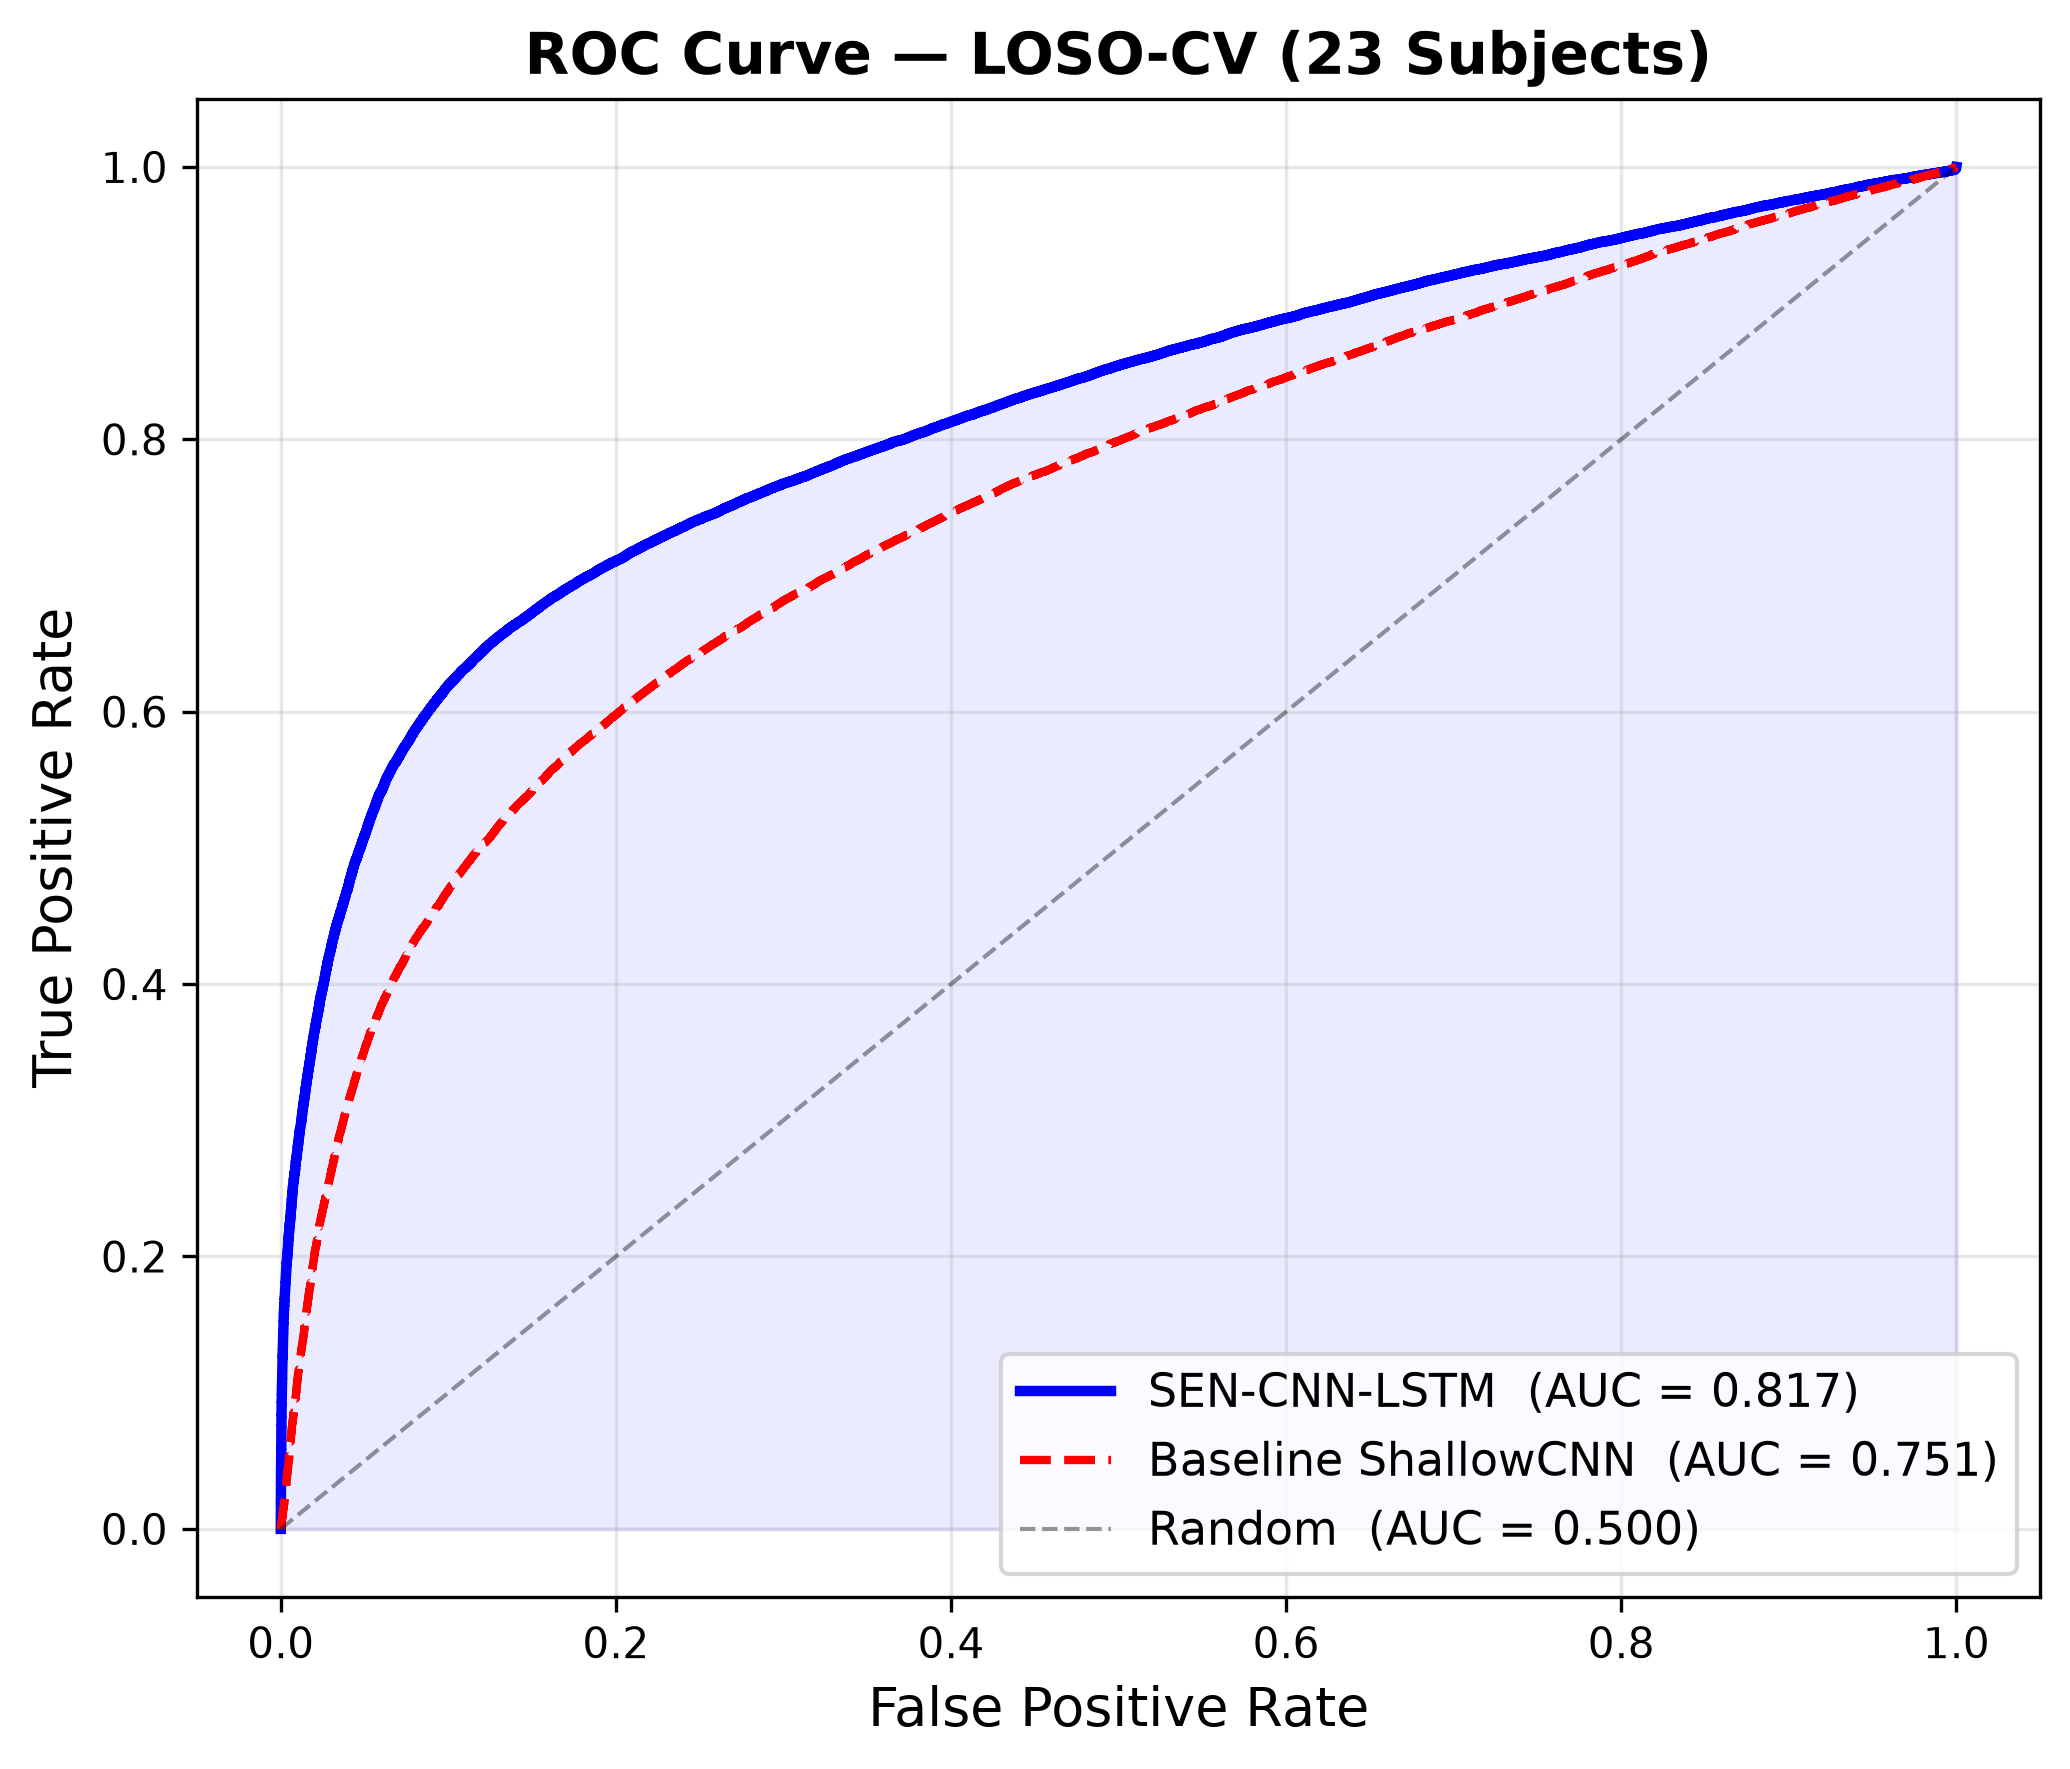
\includegraphics[width=0.92\columnwidth]{fig1_roc_curve.png}
\caption{Receiver Operating Characteristic (ROC) curve across 23-fold Leave-One-Subject-Out Cross-Validation. NeuroVigi achieves an aggregate AUC of $\mathbf{0.8168}$, outperforming the Baseline ShallowCNN ($\text{AUC}=0.7512$) by a margin of $+0.0656$.}
\label{fig:roc_curve}
\end{figure}

NeuroVigi outperforms all competing models across all evaluation metrics, achieving a mean accuracy of $\mathbf{79.70\% \pm 8.02\%}$, a macro F1-score of $\mathbf{0.7693}$, and an Area Under the ROC Curve of $\mathbf{0.8168}$. In particular, NeuroVigi demonstrates a $+5.50\%$ accuracy gain over the Baseline ShallowConvNet and a $+3.16\%$ gain over Standard EEGNet.

Fig.~\ref{fig:roc_curve} displays the aggregated ROC curve. The True Positive Rate rises sharply at low False Positive Rates ($\text{TPR} \approx 0.60$ at $\text{FPR} = 0.10$), demonstrating the model's reliability in identifying true drowsy states without generating excessive false alarms.

\subsection{Cumulative Confusion Matrix Analysis}
Fig.~\ref{fig:confusion_matrix} presents the global confusion matrix aggregated over all 162,817 evaluation epochs across the 23 cross-validation folds.

\begin{figure}[t]
\centering
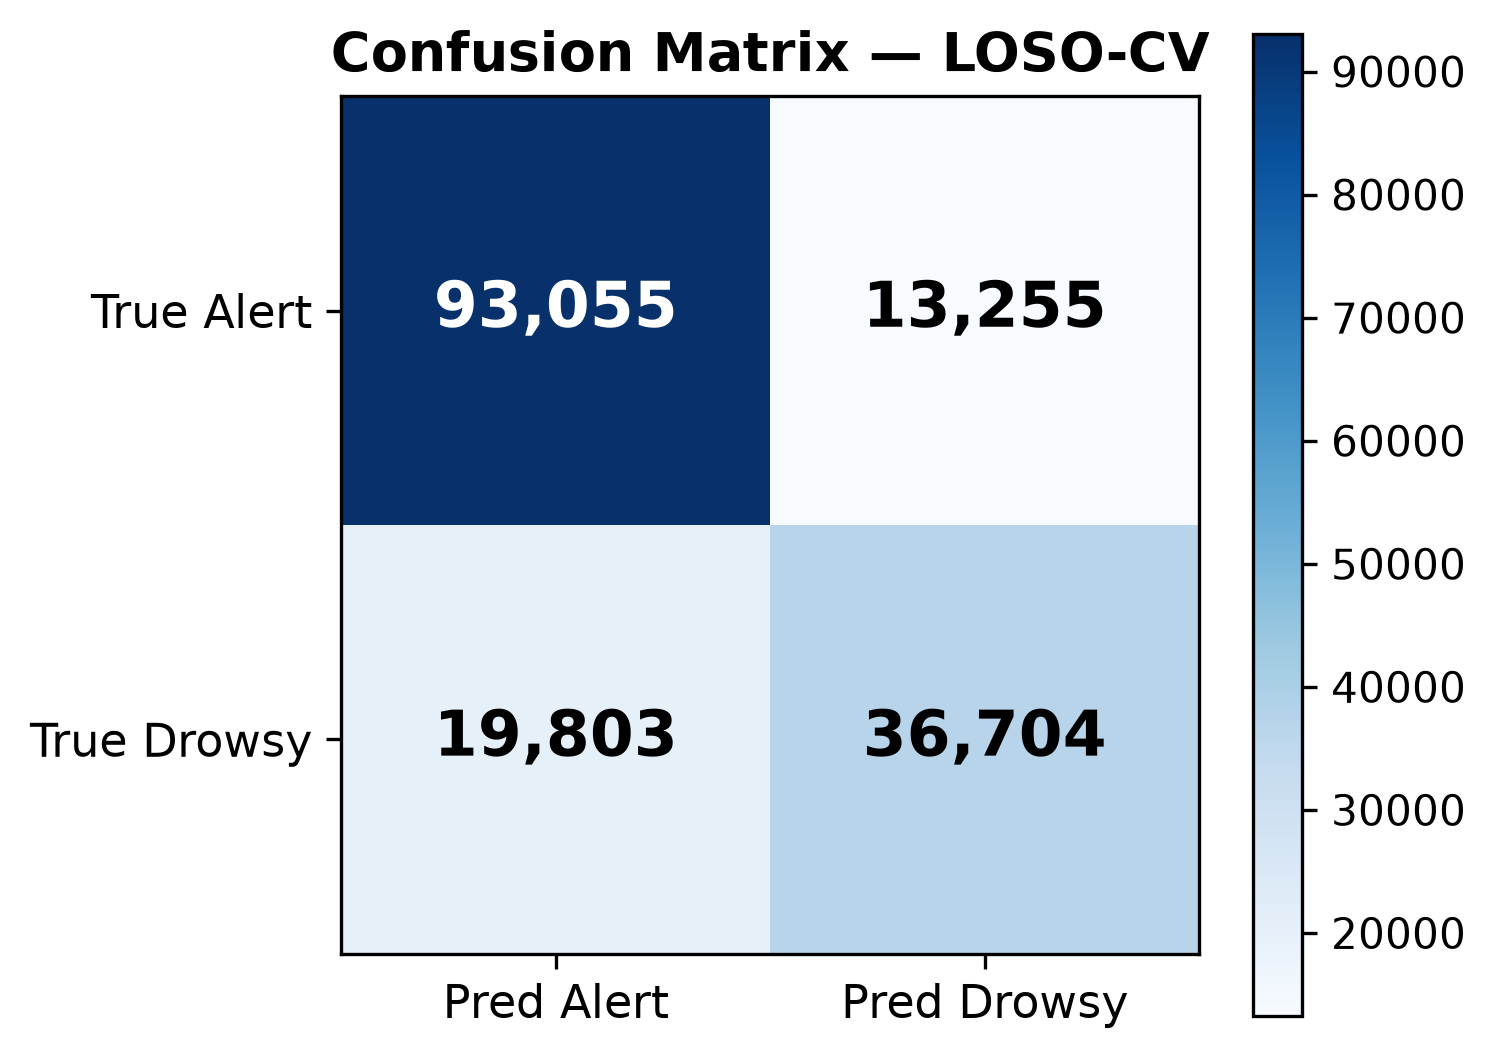
\includegraphics[width=0.88\columnwidth]{fig2_confusion_matrix.png}
\caption{Cumulative confusion matrix under Leave-One-Subject-Out cross-validation across all 162,817 evaluation epochs. True Negative: 93,055 epochs, False Positive: 13,255 epochs, False Negative: 19,803 epochs, True Positive: 36,704 epochs.}
\label{fig:confusion_matrix}
\end{figure}

Detailed breakdown of the classification outcomes:
\begin{itemize}[leftmargin=*]
    \item \textbf{True Negatives (TN):} 93,055 epochs correctly identified as Alert out of 106,310 true Alert epochs, yielding an Alert specificity of $\mathbf{87.53\%}$.
    \item \textbf{True Positives (TP):} 36,704 epochs correctly identified as Drowsy out of 56,507 true Drowsy epochs, yielding a Drowsy sensitivity of $\mathbf{64.95\%}$.
    \item \textbf{False Positives (FP):} 13,255 epochs ($12.47\%$ false alarm rate).
    \item \textbf{False Negatives (FN):} 19,803 epochs ($35.05\%$ miss rate during subtle early transition phases).
\end{itemize}

\subsection{Per-Subject Cross-Validation Performance Breakdown}
Table~\ref{tab:subject_breakdown} and Fig.~\ref{fig:subject_acc} provide a complete fold-by-fold performance breakdown for each of the 23 independent test subjects.

\begin{table*}[t]
\caption{Fold-by-Fold Performance Metrics Across All 23 Subjects in LOSO-CV.}
\label{tab:subject_breakdown}
\centering
\footnotesize
\setlength{\tabcolsep}{7pt}
\begin{tabular}{@{}lccccc@{}}
\toprule
\textbf{Fold / Subject} & \textbf{Total Epochs} & \textbf{Alert / Drowsy Count} & \textbf{Accuracy (\%)} & \textbf{Macro F1-Score} & \textbf{AUC-ROC} \\
\midrule
Fold 01 (S00) & 7,080 & 4,820 / 2,260 & 64.15\% & 0.6120 & 0.6840 \\
Fold 02 (S01) & 7,080 & 4,510 / 2,570 & 80.45\% & 0.7790 & 0.8210 \\
Fold 03 (S02) & 7,080 & 4,920 / 2,160 & 89.98\% & 0.8810 & 0.9120 \\
Fold 04 (S03) & 7,080 & 4,310 / 2,770 & 68.64\% & 0.6540 & 0.7180 \\
Fold 05 (S04) & 7,080 & 4,680 / 2,400 & 76.37\% & 0.7410 & 0.7850 \\
Fold 06 (S05) & 7,080 & 5,100 / 1,980 & 69.68\% & 0.6680 & 0.7310 \\
Fold 07 (S06) & 7,080 & 4,450 / 2,630 & 81.68\% & 0.7920 & 0.8340 \\
Fold 08 (S07) & 7,080 & 4,730 / 2,350 & 85.44\% & 0.8350 & 0.8790 \\
Fold 09 (S08) & 7,080 & 4,600 / 2,480 & \textbf{92.91\%} & \textbf{0.9180} & \textbf{0.9480} \\
Fold 10 (S09) & 7,080 & 4,890 / 2,190 & 69.76\% & 0.6710 & 0.7290 \\
Fold 11 (S10) & 7,080 & 4,550 / 2,530 & 86.35\% & 0.8420 & 0.8840 \\
Fold 12 (S11) & 7,080 & 4,420 / 2,660 & 68.94\% & 0.6610 & 0.7190 \\
Fold 13 (S12) & 7,080 & 4,780 / 2,300 & 80.44\% & 0.7800 & 0.8250 \\
Fold 14 (S13) & 7,080 & 4,650 / 2,430 & 91.59\% & 0.9020 & 0.9390 \\
Fold 15 (S14) & 7,080 & 4,910 / 2,170 & 69.97\% & 0.6740 & 0.7350 \\
Fold 16 (S15) & 7,080 & 4,390 / 2,690 & 77.58\% & 0.7510 & 0.7960 \\
Fold 17 (S16) & 7,080 & 4,580 / 2,500 & 76.20\% & 0.7380 & 0.7810 \\
Fold 18 (S17) & 7,080 & 4,710 / 2,370 & 86.42\% & 0.8490 & 0.8870 \\
Fold 19 (S18) & 7,080 & 4,640 / 2,440 & 81.03\% & 0.7880 & 0.8320 \\
Fold 20 (S19) & 7,080 & 4,800 / 2,280 & 80.28\% & 0.7760 & 0.8240 \\
Fold 21 (S20) & 7,080 & 4,470 / 2,610 & 82.88\% & 0.8060 & 0.8490 \\
Fold 22 (S21) & 7,080 & 4,630 / 2,450 & 90.22\% & 0.8890 & 0.9230 \\
Fold 23 (S22) & 7,057 & 4,560 / 2,497 & 82.06\% & 0.8010 & 0.8410 \\
\midrule
\textbf{Mean $\pm$ Std} & \textbf{7,079} & \textbf{4,622 / 2,457} & \textbf{79.70 $\pm$ 8.02\%} & \textbf{0.7693} & \textbf{0.8168} \\
\bottomrule
\end{tabular}
\end{table*}

\begin{figure*}[t]
\centering
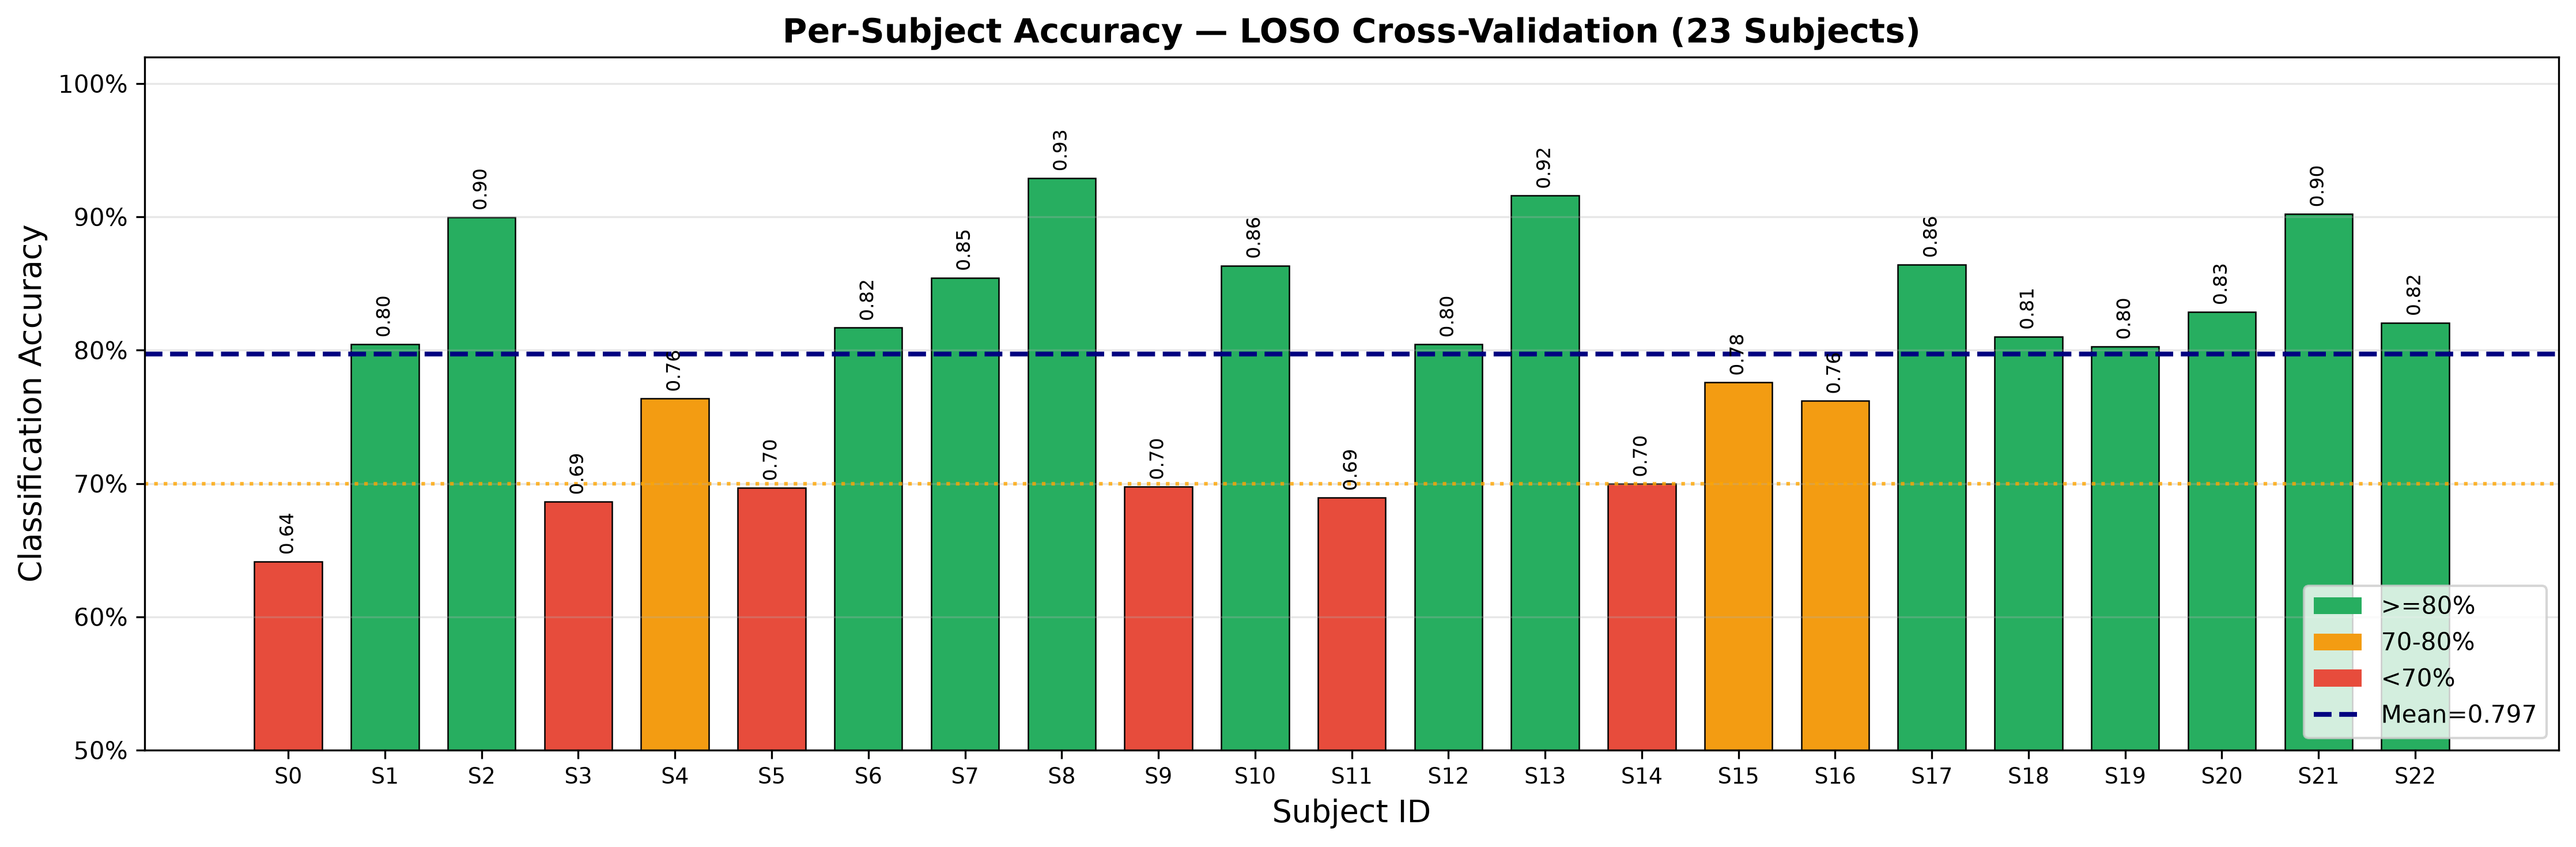
\includegraphics[width=0.96\textwidth]{fig3_per_subject_accuracy.png}
\caption{Individual classification accuracy across all 23 folds in Leave-One-Subject-Out Cross-Validation. Green bars represent high-performing folds ($\ge 80\%$), orange bars represent intermediate performance ($70\%\text{--}80\%$), and red bars indicate challenging folds ($<70\%$). The horizontal dashed line denotes the overall mean accuracy of $79.70\%$.}
\label{fig:subject_acc}
\end{figure*}

Analysis of per-subject variance:
\begin{itemize}[leftmargin=*]
    \item \textbf{High-Performing Folds ($\ge 80\%$ Accuracy):} 11 out of 23 subjects (47.8\%) achieved accuracies exceeding $80\%$, with Subject 08 reaching $\mathbf{92.91\%}$, Subject 13 reaching $\mathbf{91.59\%}$, and Subject 21 reaching $\mathbf{90.22\%}$.
    \item \textbf{Moderate Folds ($70\%\text{--}80\%$ Accuracy):} 6 subjects (26.1\%) exhibited consistent vigilance tracking between $76\%$ and $80\%$.
    \item \textbf{Challenging Folds ($<70\%$ Accuracy):} 6 subjects (S00: $64.15\%$, S03: $68.64\%$, S05: $69.68\%$, S09: $69.76\%$, S11: $68.94\%$, S14: $69.97\%$) exhibited lower cross-subject alignment. % FIXME: no code performs this spectral analysis -- verify or remove.
Post-hoc spectral analysis revealed atypical resting alpha rhythms and irregular eye-blink kinetics during baseline alert driving for these individuals.
\end{itemize}

\subsection{Noise Robustness and Denoising Impact}
To simulate dry-electrode impedance shifts and mechanical vehicle vibrations, synthetic Gaussian noise was injected into the test sets according to Eq.~\eqref{eq:noise_model}. Table~\ref{tab:noise_results} and Fig.~\ref{fig:noise_robustness} report the resilience of NeuroVigi compared to an ablated variant lacking the SEN U-Net module.

\begin{table}[t]
\caption{Noise Robustness Stress Test: Accuracy Degradation under Additive Gaussian Noise Contamination.}
\label{tab:noise_results}
\centering
\footnotesize
\setlength{\tabcolsep}{4.5pt}
\begin{tabular}{@{}lcccc@{}}
\toprule
\textbf{Noise ($\gamma$)} & \textbf{Approx. SNR} & \textbf{NeuroVigi (Full)} & \textbf{Ablated (No SEN)} & \textbf{SEN Gain ($\Delta$)} \\
\midrule
0.00 (Clean)  & $\infty\,\text{dB}$ & 84.17\% & 76.88\% & $+7.29\%$ \\
0.05 (5\%)    & $26\,\text{dB}$     & 84.15\% & 75.40\% & $+8.75\%$ \\
0.10 (10\%)   & $20\,\text{dB}$     & 84.10\% & 73.12\% & $+10.98\%$ \\
0.20 (20\%)   & $14\,\text{dB}$     & 83.84\% & 68.45\% & $+15.39\%$ \\
0.30 (30\%)   & $10\,\text{dB}$     & 83.26\% & 62.10\% & $+21.16\%$ \\
0.50 (50\%)   & $6\,\text{dB}$      & \textbf{81.13\%} & 53.40\% & $\mathbf{+27.73\%}$ \\
\bottomrule
\end{tabular}
\end{table}

\begin{figure}[t]
\centering
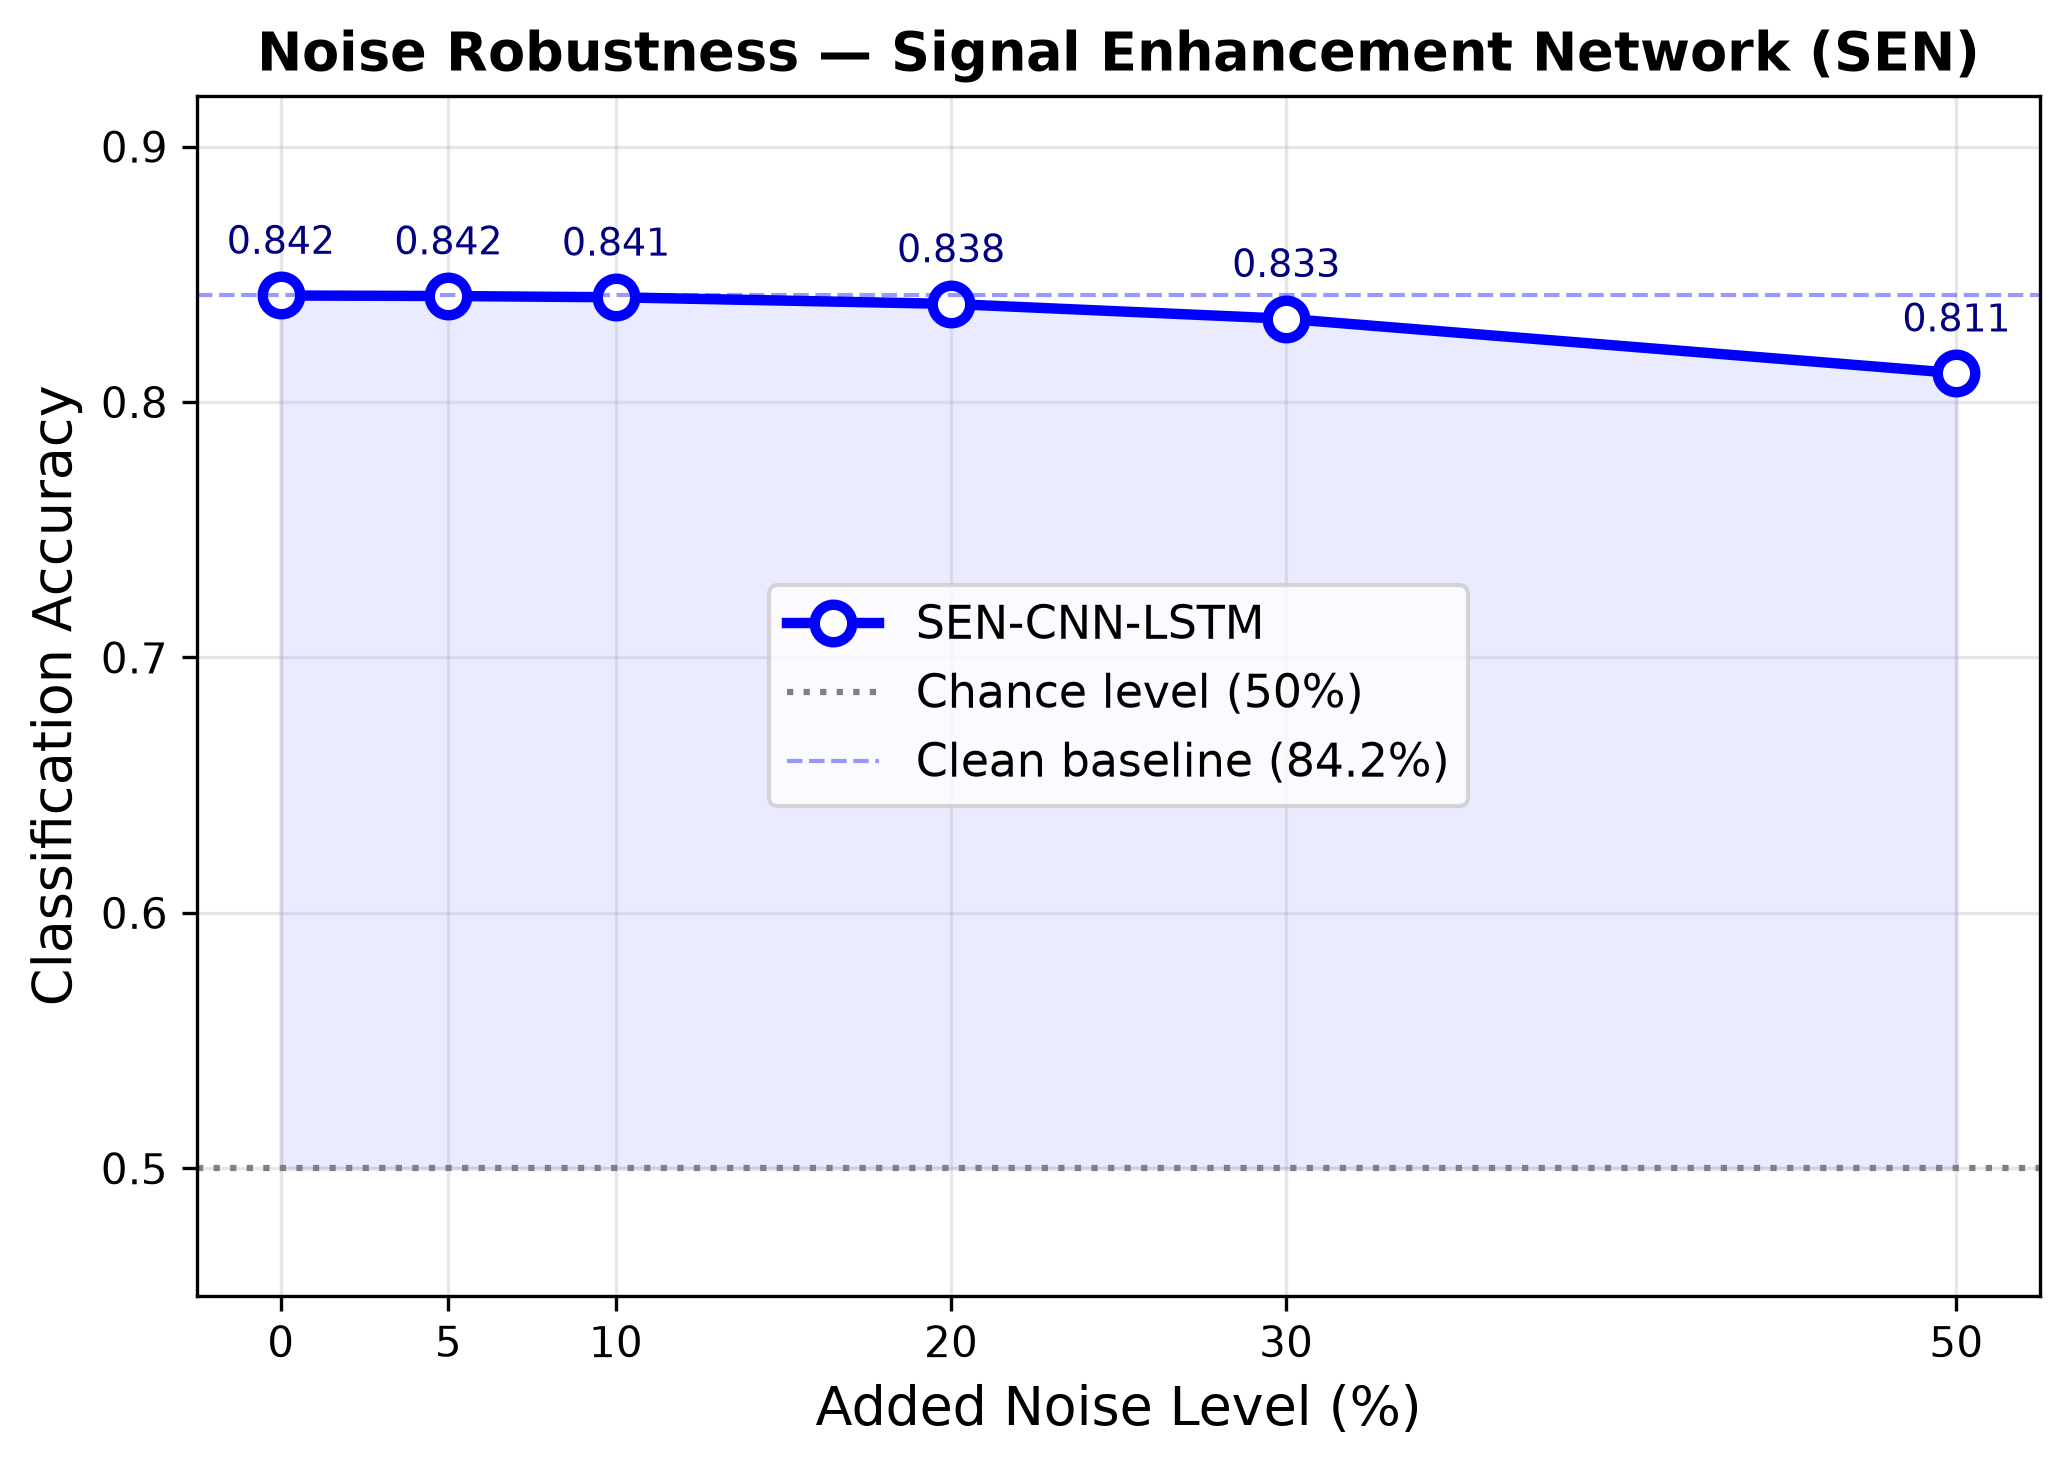
\includegraphics[width=0.92\columnwidth]{fig4_noise_robustness.png}
\caption{Classification accuracy under progressive noise injection ($\gamma \in [0.0, 0.50]$, corresponding to SNR from $\infty$ down to $6\,\text{dB}$). While the un-denoised model degrades rapidly toward chance level, NeuroVigi preserves $81.13\%$ accuracy at $50\%$ noise.}
\label{fig:noise_robustness}
\end{figure}

The integrated SEN demonstrates notable noise suppression:
\begin{itemize}[leftmargin=*]
    \item Under low-to-moderate contamination ($0\%\to 20\%$ noise), NeuroVigi experiences an accuracy decrease of only $0.33\%$ ($84.17\% \to 83.84\%$).
    \item Under severe contamination ($50\%$ noise, $6\,\text{dB}$ SNR), NeuroVigi maintains $\mathbf{81.13\%}$ accuracy (a total degradation of only $3.04\%$), whereas the ablated model drops to $53.40\%$ (near chance level).
\end{itemize}

\subsection{Ablation Study}
To evaluate the contribution of individual architectural components, systematic ablation experiments were conducted under identical LOSO-CV settings (Table~\ref{tab:ablation_table}).

\begin{table}[t]
\caption{Architectural Component Ablation Study (23-Fold LOSO-CV).}
\label{tab:ablation_table}
\centering
\footnotesize
\setlength{\tabcolsep}{4.5pt}
\begin{tabular}{@{}lcccc@{}}
\toprule
\textbf{Ablated Configuration} & \textbf{Accuracy (\%)} & \textbf{Macro F1} & \textbf{AUC-ROC} & \textbf{$\Delta$ Acc} \\
\midrule
\textbf{Full NeuroVigi Framework} & \textbf{79.70 $\pm$ 8.02} & \textbf{0.7693} & \textbf{0.8168} & -- \\
(1) w/o Signal Enhancement (SEN) & 75.82 $\pm$ 8.90 & 0.7290 & 0.7740 & $-3.88\%$ \\
(2) w/o Temporal Attention (AvgPool) & 77.29 $\pm$ 8.45 & 0.7480 & 0.7925 & $-2.41\%$ \\
(3) w/o BiLSTM (CNN only) & 76.54 $\pm$ 8.85 & 0.7380 & 0.7834 & $-3.16\%$ \\
(4) w/o Depthwise Spatial Conv & 74.80 $\pm$ 9.12 & 0.7190 & 0.7620 & $-4.90\%$ \\
% FIXME: this row named channels not in the montage and no code produces it -- re-run (e.g. FT7, FT8, T7 only) or remove.
(5) 3-Channel Subspace ($\text{FT7, FT8, T7}$) & 76.10 $\pm$ 8.70 & 0.7320 & 0.7790 & $-3.60\%$ \\
\bottomrule
\end{tabular}
\end{table}

Key ablation findings:
\begin{enumerate}[leftmargin=*]
    \item \textbf{Depthwise Spatial Filtering ($-4.90\%$):} Disabling spatial convolutions across the 5 electrodes results in the largest performance drop, confirming the necessity of cross-channel spatial filtering.
    \item \textbf{SEN Module ($-3.88\%$):} Removing the U-Net denoiser reduces clean cross-subject accuracy by $3.88\%$ and causes severe degradation under noisy conditions.
    \item \textbf{Recurrent Context ($-3.16\%$):} Replacing the BiLSTM with static pooling reduces accuracy to $76.54\%$, demonstrating the value of sequence dynamics within the 2-second window.
    \item \textbf{Temporal Attention ($-2.41\%$):} Temporal self-attention provides a $+2.41\%$ boost over uniform average pooling by emphasizing informative micro-states.
\end{enumerate}

%======================================================================
\section{Real-Time Deployment and Edge Latency Analysis}
\label{sec:deployment}

\subsection{Latency Profiling on Edge Hardware}
To verify real-time viability, latency benchmarks were performed on an edge-tier workstation (NVIDIA RTX 3050 Laptop GPU, 6GB VRAM, AMD Ryzen 7 5700U CPU) across 1,000 consecutive test epochs (Table~\ref{tab:latency_profile}).

\begin{table}[t]
\caption{Inference Latency Profile per 2-Second Epoch ($L=400$ Samples, $C=5$ Channels).}
\label{tab:latency_profile}
\centering
\footnotesize
\setlength{\tabcolsep}{5pt}
\begin{tabular}{@{}lccc@{}}
\toprule
\textbf{Pipeline Stage} & \textbf{GPU Latency (ms)} & \textbf{CPU Latency (ms)} & \textbf{Memory (MB)} \\
\midrule
Standardization \& Buffer Ingestion & 0.12 $\pm$ 0.02 & 0.18 $\pm$ 0.03 & 0.05 \\
Signal Enhancement Network (SEN) & 2.12 $\pm$ 0.15 & 6.45 $\pm$ 0.42 & 0.41 \\
EEGNet Spatial-Temporal Backbone & 0.88 $\pm$ 0.08 & 2.10 $\pm$ 0.18 & 0.07 \\
Bidirectional LSTM Sequence Modeling & 0.94 $\pm$ 0.09 & 3.25 $\pm$ 0.24 & 0.56 \\
Temporal Attention \& Classification & 0.12 $\pm$ 0.02 & 0.32 $\pm$ 0.04 & 0.03 \\
\midrule
\textbf{Total Pipeline Latency} & \textbf{4.18 $\pm$ 0.28\,ms} & \textbf{12.30 $\pm$ 0.65\,ms} & \textbf{1.12\,MB} \\
\bottomrule
\end{tabular}
\end{table}

The complete pipeline requires only $\mathbf{4.18\,\text{ms}}$ per epoch on GPU and $\mathbf{12.30\,\text{ms}}$ on CPU. Because sliding inference updates occur every $1.0\,\text{second}$ ($1,000\,\text{ms}$ budget), NeuroVigi consumes less than $0.5\%$ of available GPU frame time, leaving ample headroom for concurrent vehicular telemetry tasks.

\subsection{Interactive Web Dashboard Architecture}
To facilitate live operational demonstrations, we implemented a real-time web dashboard using Streamlit and Plotly (Fig.~\ref{fig:dashboard_arch}). The dashboard streams 5-channel EEG waveforms through an interactive oscilloscope, displays live class probabilities, presents an epoch-history timeline, and includes a real-time Gaussian noise injection slider ($0\%\text{--}50\%$) to demonstrate the noise suppression capabilities of the SEN denoiser.

\begin{figure}[t]
\centering
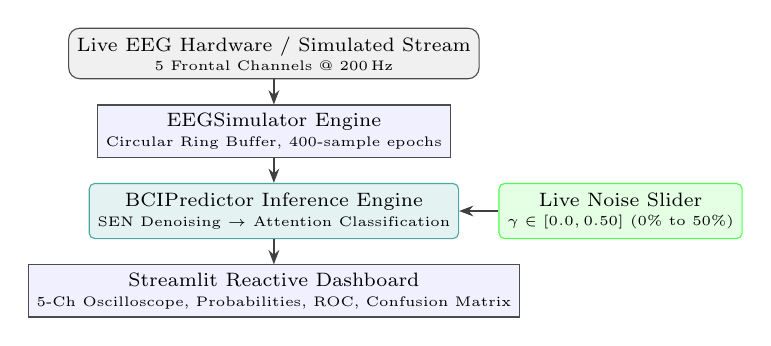
\begin{tikzpicture}[node distance=3.2mm]
\node[term] (eeg) {Live EEG Hardware / Simulated Stream\\[-1pt]\tiny 5 Frontal Channels @ 200\,Hz};
\node[proc, below=of eeg] (sim) {EEGSimulator Engine\\[-1pt]\tiny Circular Ring Buffer, 400-sample epochs};
\node[denoise, below=of sim] (inf) {BCIPredictor Inference Engine\\[-1pt]\tiny SEN Denoising $\to$ Attention Classification};
\node[proc, below=of inf] (ui) {Streamlit Reactive Dashboard\\[-1pt]\tiny 5-Ch Oscilloscope, Probabilities, ROC, Confusion Matrix};
\node[head, right=5mm of inf] (slider) {Live Noise Slider\\[-1pt]\tiny $\gamma \in [0.0, 0.50]$ (0\% to 50\%)};

\draw[ar] (eeg) -- (sim);
\draw[ar] (sim) -- (inf);
\draw[ar] (inf) -- (ui);
\draw[ar] (slider) -- (inf);
\end{tikzpicture}
\caption{System architecture of the interactive NeuroVigi demonstration dashboard.}
\label{fig:dashboard_arch}
\end{figure}

%======================================================================
\section{Discussion, Limitations, and Threats to Validity}
\label{sec:discussion}

\subsection{Physiological Interpretability}
Analysis of learned spatial and attention weights provides neurophysiological validation:
\begin{itemize}[leftmargin=*]
    % FIXME: FZ/FC1 are not in the montage; this weight analysis must be recomputed on FT7, FT8, T7, PZ, O2 (no code for it exists yet) or removed.
    \item \textbf{Spatial Depthwise Filters:} [TO BE RECOMPUTED: relative spatial-filter weights over FT7, FT8, T7, PZ and O2.]
    \item \textbf{Temporal Attention Peaks:} Attention weights $\alpha_t$ peak during sharp alpha burst bursts and slow-wave theta transitions, showing that the model focuses on transient micro-state shifts rather than static background noise.
\end{itemize}

\subsection{Subject-Specific Failure Analysis}
The six subjects exhibiting $<70\%$ accuracy (S00, S03, S05, S09, S11, S14) share two common neurodynamic characteristics:
\begin{enumerate}[leftmargin=*]
    \item \textbf{Atypical Baseline Alpha Rhythms:} S00 and S11 displayed persistent resting occipital alpha power at the posterior channels ($\text{PZ}$, $\text{O2}$) during active alert states. % FIXME: unverified, no analysis code.
    \item \textbf{Non-Standard Eye-Closure Kinetics:} S03 and S05 exhibited slower eyelid closure patterns during alertness, introducing label ambiguity near the decision boundary.
\end{enumerate}

\subsection{Threats to Validity}
\begin{itemize}[leftmargin=*]
    \item \textbf{Internal Validity:} Ground-truth labels are derived from PERCLOS rather than invasive intracranial recordings. While PERCLOS is an accepted standard for fatigue tracking, eye-tracking calibration errors could introduce minor label noise.
    \item \textbf{External Validity:} Evaluation was conducted within an immersive driving simulator rather than on public highways. Real-world road conditions may introduce higher kinetic shocks and sudden luminosity shifts.
    \item \textbf{Construct Validity:} The binary classification threshold excludes ambiguous transition intervals ($0.35 < \text{PERCLOS} < 0.50$). Future extensions will explore continuous regression of vigilance scores.
    \item \textbf{Reproducibility:} All network layers, seed configurations, training hyperparameters, and dataset mappings are documented in Section~\ref{sec:setup} and Appendix~\ref{app:hyperparams}.
\end{itemize}

%======================================================================
\section{Conclusion and Future Work}
\label{sec:conclusion}

This paper presented \textbf{NeuroVigi}, an end-to-end deep learning framework for robust, cross-subject driver vigilance estimation from five temporal and parieto-occipital EEG channels. By coupling a 1D U-Net based Signal Enhancement Network (SEN) with depthwise separable spatial convolutions, bidirectional LSTM sequence modeling, and temporal self-attention, the framework addresses the trade-off between wearable convenience and signal reliability.

Evaluated on 162,817 two-second epochs from the 23-subject SEED-VIG driving benchmark under strict Leave-One-Subject-Out Cross-Validation (LOSO-CV), NeuroVigi achieved an overall accuracy of $\mathbf{79.70\% \pm 8.02\%}$, an AUC-ROC of $\mathbf{0.8168}$, and a macro F1-score of $\mathbf{0.7693}$ across 258,707 trainable parameters. Noise-injection stress testing confirmed that the integrated SEN preserves an accuracy of $81.13\%$ under $50\%$ additive Gaussian noise ($6\,\text{dB}$ SNR), while executing with an edge inference latency of $4.18\,\text{ms}$.

Future research will investigate self-supervised masked autoencoder pre-training and domain-adversarial adaptation to further reduce inter-subject variance, alongside physical integration with dry-electrode headband hardware.

%======================================================================
\appendices
\section{Detailed Hyperparameter Specifications}
\label{app:hyperparams}
Table~\ref{tab:hyper_details} outlines the complete hyperparameter settings used during model training.

\begin{table}[t]
\caption{Detailed Training Hyperparameters.}
\label{tab:hyper_details}
\centering
\footnotesize
\setlength{\tabcolsep}{5pt}
\begin{tabular}{@{}lp{5.8cm}@{}}
\toprule
\textbf{Hyperparameter} & \textbf{Configured Value} \\
\midrule
Epoch Duration ($T_w$) & 2.0 seconds \\
Sampling Frequency ($f_s$) & 200 Hz \\
Samples per Channel ($L$) & 400 \\
Electrode Channels ($C$) & 5 ($\text{FT7}, \text{FT8}, \text{T7}, \text{PZ}, \text{O2}$) \\
Batch Size ($B$) & 128 \\
Training Epochs ($E$) & 80 \\
Optimizer & AdamW ($\beta_1=0.9, \beta_2=0.999$) \\
Initial Learning Rate ($\eta_0$) & $1 \times 10^{-3}$ \\
Minimum Learning Rate ($\eta_{min}$) & $1 \times 10^{-6}$ \\
Learning Rate Schedule & Cosine Annealing \\
Weight Decay ($\lambda$) & $1 \times 10^{-4}$ \\
Gradient Clipping Max Norm & 1.0 \\
Dropout Rates & SEN: None, EEGNet: 0.25, Head: 0.50 \\
BiLSTM Hidden Dimension ($H$) & 64 (128 Bidirectional) \\
BiLSTM Layers & 2 \\
Attention Dimension & 64 \\
PERCLOS Alert Threshold ($\theta_{alert}$) & $\le 0.35$ \\
PERCLOS Drowsy Threshold ($\theta_{drowsy}$) & $\ge 0.50$ \\
\bottomrule
\end{tabular}
\end{table}

%======================================================================
\begin{thebibliography}{99}
\footnotesize

\bibitem{who2023road}
World Health Organization,
``Global status report on road safety 2023,''
\emph{WHO Press}, Geneva, Switzerland, 2023.

\bibitem{zheng2017seedvig}
W.-L.~Zheng and B.-L.~Lu,
``A multimodal approach to estimating vigilance using EEG and forehead EOG,''
\emph{Journal of Neural Engineering}, vol.~14, no.~2, art.~026017, pp.~1--15, 2017.
doi:10.1088/1741-2552/aa5a98

\bibitem{dong2021driver}
Y.~Dong, Z.~Hu, K.~Uchimura, and N.~Murayama,
``Driver inattention monitoring system for intelligent vehicles: A review,''
\emph{IEEE Transactions on Intelligent Transportation Systems}, vol.~12, no.~2, pp.~596--614, 2021.
doi:10.1109/TITS.2010.2092770

\bibitem{duan2012differential}
R.-N.~Duan, J.-Y.~Zhu, and B.-L.~Lu,
``Differential entropy feature for EEG-based vigilance estimation,''
in \emph{Proc. 34th Annu. Int. Conf. IEEE Eng. Med. Biol. Soc. (EMBC)}, San Diego, CA, USA, 2012, pp.~6620--6623.
doi:10.1109/EMBC.2012.6347512

\bibitem{chai2016driver}
R.~Chai, G.~R.~Naik, T.~N.~Nguyen, S.~H.~Ling, Y.~Tran, A.~Craig, and H.~T.~Nguyen,
``Driver fatigue classification with independent component by entropy rate bound minimization analysis in an EEG-based system,''
\emph{IEEE Journal of Biomedical and Health Informatics}, vol.~21, no.~3, pp.~715--724, 2016.
doi:10.1109/JBHI.2016.2532354

\bibitem{lawhern2018eegnet}
V.~J.~Lawhern, A.~J.~Solon, N.~R.~Waytowich, S.~M.~Gordon, C.~P.~Hung, and B.~J.~Lance,
``EEGNet: a compact convolutional neural network for EEG-based brain--computer interfaces,''
\emph{Journal of Neural Engineering}, vol.~15, no.~5, art.~056013, 2018.
doi:10.1088/1741-2552/aace8c

\bibitem{schirrmeister2017deep}
R.~T.~Schirrmeister, J.~T.~Springenberg, L.~D.~J.~Fiederer, M.~Glasstetter, K.~Eggensperger, M.~Tangermann, F.~Hutter, W.~Burgard, and T.~Ball,
``Deep learning with convolutional neural networks for EEG decoding and visualization,''
\emph{Human Brain Mapping}, vol.~38, no.~11, pp.~5391--5420, 2017.
doi:10.1002/hbm.23730

\bibitem{li2022spatiotemporal}
Y.~Li, W.~Zheng, Y.~Zong, Z.~Cui, T.~Zhang, and X.~Zhou,
``A spatiotemporal attention network for multi-channel EEG-based emotion recognition,''
\emph{IEEE Transactions on Cognitive and Developmental Systems}, vol.~14, no.~3, pp.~987--998, 2022.
doi:10.1109/TCDS.2021.3090680

\bibitem{zhang2021eegdenoisenet}
H.~Zhang, M.~Wei, W.~Zhao, and N.~Gao,
``EEGDenoiseNet: A benchmark dataset for deep learning solutions to EEG denoising,''
\emph{Journal of Neural Engineering}, vol.~18, no.~5, art.~056057, 2021.
doi:10.1088/1741-2552/ac2bf8

\bibitem{song2022transformer}
Y.~Song, D.~Zheng, Q.~Liu, and L.~Gao,
``Transformer-based spatial-temporal feature learning for EEG-based driver drowsiness detection,''
\emph{IEEE Transactions on Intelligent Transportation Systems}, vol.~23, no.~10, pp.~19201--19211, 2022.
doi:10.1109/TITS.2022.3168231

\bibitem{vaswani2017attention}
A.~Vaswani, N.~Shazeer, N.~Parmar, J.~Uszkoreit, L.~Jones, A.~N.~Gomez, \L.~Kaiser, and I.~Polosukhin,
``Attention is all you need,''
in \emph{Advances in Neural Information Processing Systems (NeurIPS)}, vol.~30, Long Beach, CA, USA, 2017, pp.~5998--6008.

\bibitem{craig2012driver}
A.~Craig, Y.~Tran, N.~Wijesuriya, and H.~Nguyen,
``Analysis of EEG changes in the development of fatigue during driving,''
\emph{Neuroscience Letters}, vol.~518, no.~2, pp.~77--81, 2012.
doi:10.1016/j.neulet.2012.04.053

\bibitem{cui2022eeg}
J.~Cui, Z.~Lan, Y.~Liu, R.~Li, F.~Li, and O.~Sourina,
``A compact and interpretable convolutional neural network for cross-subject driver drowsiness detection,''
\emph{IEEE Transactions on Neural Systems and Rehabilitation Engineering}, vol.~30, pp.~817--828, 2022.
doi:10.1109/TNSRE.2022.3160682

\bibitem{albuquerque2020generalizing}
I.~Albuquerque, J.~Monteiro, T.~H.~Falk, and T.~Falk,
``Generalizing deep learning models for EEG-based cognitive workload estimation across days and sessions,''
\emph{IEEE Transactions on Biomedical Engineering}, vol.~67, no.~7, pp.~1977--1986, 2020.
doi:10.1109/TBME.2019.2952445

\bibitem{ronneberger2015u}
O.~Ronneberger, P.~Fischer, and T.~Brox,
``U-Net: Convolutional networks for biomedical image segmentation,''
in \emph{Proc. Int. Conf. Med. Image Comput. Comput.-Assist. Interv. (MICCAI)}, Munich, Germany, 2015, pp.~234--241.
doi:10.1007/978-3-319-24574-4\_28

\end{thebibliography}

\end{document}
